%----------------------------------------------------------------------------------------------------------------------------
\graphicspath{{Parti/P03-Meccanica_SR/C07-Classificazione_SCR/Figure/}}
\chapter{Classificazione dei sistemi di corpi rigidi}\label{cap:classificazione_SCR}
%----------------------------------------------------------------------------------------------------------------------------

\begin{sommario}
	Si sviluppano gli strumenti per riconoscere e classificare 
	i sistemi di corpi rigidi piani vincolati. Il conteggio 
	dei gradi di libertà nominali $\nu = 3n_c - m$ costituisce 
	un criterio necessario ma non sufficiente: esso fissa le 
	dimensioni della matrice di congruenza $\bm{A}$ senza 
	determinarne il rango, sicché a parità di $\nu$ la 
	disposizione geometrica dei vincoli può produrre 
	classificazioni diverse. Si richiama il calcolo di $m$ 
	dalle molteplicità dei vincoli elementari, con il vincolo 
	di rigidità come caso limite che consente di fondere 
	corpi collegati rigidamente in un unico corpo equivalente, 
	e si introduce la distinzione fra isostaticità globale 
	e locale. Il nucleo del capitolo è il catalogo delle 
	sottostrutture elementari più frequenti --- da un singolo 
	corpo fino a tre corpi --- nel quale i casi regolari e 
	degeneri sono affiancati e le cause geometriche della 
	degenerazione --- parallelismo o concorrenza degli assi 
	di vincolo, allineamento dei centri di rotazione --- 
	sono identificate e interpretate. Il catalogo abilita 
	la classificazione per decomposizione gerarchica e per 
	riduzione a schema noto, e si raccorda con le strategie 
	di soluzione del \CAPref{cap:classificazione_sol_SCR}.
\end{sommario}



%----------------------------------------------------------------------------------------------------------------------------
\section{Il conteggio come criterio necessario}
\label{sec:conteggio_necessario}
%----------------------------------------------------------------------------------------------------------------------------

Nel \CAPref{cap:problemi_cin_stat_SCR} si è mostrato che la
classificazione di un sistema di $n_c$ corpi rigidi piani vincolati
da $m$ equazioni scalari dipende dal rango della matrice dei
vincoli $\bm{A} \in \mathbb{R}^{m \times n}$, con $n = 3n_c$.
La formula fondamentale
\begin{equation}\label{eq:formula_class_richiamo}
	g_\ell - g_{\mathscr{i}} = n - m = 3n_c - m \eqqcolon \nu
\end{equation}
lega il grado di labilità $g_\ell = \nl(\bm{A})$ e il grado di
iperstaticità $g_{\mathscr{i}} = \nl(\bm{A}^\top)$ alla
differenza $\nu = 3n_c - m$, calcolabile a priori dal solo
conteggio dei corpi e dei vincoli scalari, senza costruire
$\bm{A}$.

Il numero $\nu$ è dunque il primo strumento di classificazione\index{classificazione dei sistemi di corpi rigidi|textbf}\index{conteggio dei gradi di libertà|textbf}:
fissa le \emph{dimensioni} di $\bm{A}$ e la differenza
$g_\ell - g_{\mathscr{i}}$, ma non determina i due gradi
separatamente. Il segno e il valore di $\nu$ individuano tre
\emph{casi nominali}:

\begin{itemize}[nosep]
	\item $\nu > 0$: il sistema ha più gradi di libertà che
	vincoli; la matrice $\bm{A}$ ha più colonne che righe
	e non può avere rango pieno per colonne. Il sistema è
	\emph{certamente labile}\index{labilita@labilità|textbf}\index{labilita@labilità|seealso{iperstaticità, meccanismo}}, con $g_\ell \geq \nu$;
	
	\item $\nu = 0$: la matrice $\bm{A}$ è quadrata; il caso
	nominale è l'isostaticità\index{isostaticita@isostaticità|textbf}\index{isostaticita@isostaticità|seealso{labilità, iperstaticità}} ($g_\ell = g_{\mathscr{i}} = 0$),
	ma non è l'unico possibile;
	
	\item $\nu < 0$: il sistema ha più vincoli che gradi di
	libertà; la matrice $\bm{A}$ ha più righe che colonne e
	non può avere rango pieno per righe. Il sistema è
	\emph{certamente iperstatico}\index{iperstaticita@iperstaticità|textbf}\index{iperstaticita@iperstaticità|seealso{labilità, stato di autoequilibrio}}, con
	$g_{\mathscr{i}} \geq |\nu|$.
\end{itemize}

Il caso $\nu = 0$ merita attenzione particolare. La condizione
necessaria per l'isostaticità è $\nu = 0$, ma essa non è
sufficiente: una matrice quadrata può essere singolare. Se la
geometria dei vincoli è degenere --- ad esempio, tutti i vincoli
hanno assi paralleli, oppure tutte le loro linee d'azione
convergono in un punto --- la matrice $\bm{A}$ perde rango pur
essendo quadrata. In questo caso $g_\ell = g_{\mathscr{i}} > 0$:
il sistema è simultaneamente labile e iperstatico. Poiché la
\eqref{eq:formula_class_richiamo} resta valida, i due gradi si
compensano a vicenda ($g_\ell = g_{\mathscr{i}}$), e il sistema
presenta meccanismi cinematici e stati di autoequilibrio in ugual
numero. Questo è il \emph{caso labile-iperstatico}, detto anche
caso \emph{degenere}\index{degenerazione geometrica}, già classificato nella
\TABref{tab:classificazione} del \CAPref{cap:problemi_cin_stat_SCR}.

\begin{oss}[Il conteggio fissa le dimensioni, non il rango]
	La quantità $\nu$ è un dato puramente \emph{topologico}: dipende
	da quanti corpi ci sono e da quanti vincoli scalari li collegano,
	non da come questi vincoli sono geometricamente disposti.
	Cambiare la posizione di un vincolo senza alterarne il numero
	di equazioni scalari lascia $\nu$ invariato ma può modificare
	$\rg(\bm{A})$, e quindi cambiare la classificazione effettiva.
	Il conteggio è quindi la porta d'ingresso
	all'analisi, non la sua conclusione.
\end{oss}

\begin{oss}[Casi $\nu \neq 0$ e degenerazione]
	Anche nei casi $\nu > 0$ e $\nu < 0$ è possibile una
	degenerazione geometrica: il rango di $\bm{A}$ può essere
	inferiore al suo minimo teorico $\min(m,n)$, producendo
	valori di $g_\ell$ e $g_{\mathscr{i}}$ entrambi superiori
	ai minimi $\nu$ e $0$ (rispettivamente). Tuttavia, poiché
	questi casi presentano già una labilità o un'iperstaticità
	strutturale garantita dal conteggio, la degenerazione
	aggiuntiva ha in pratica minor rilevanza progettuale. Il
	caso più delicato --- e il più frequente nella pratica ---
	rimane $\nu = 0$ con degenerazione geometrica.
\end{oss}

Il programma di questo capitolo è di sviluppare strumenti
per decidere il caso effettivo senza costruire $\bm{A}$
esplicitamente. Si procederà in tre passi: prima si stabilirà
come calcolare $m$ in modo sistematico a partire dalla geometria
del sistema (\PARref{sec:conteggio_m}); poi si introdurrà la
distinzione tra comportamento globale e locale
(\PARref{sec:rigidita_interna}--\ref{sec:globale_locale});
infine si svilupperà il catalogo delle sottostrutture elementari
con i criteri di decomposizione e riduzione
(\PARref{sec:catalogo}), che si sintetizzano nella procedura
di ispezione diretta (\PARref{sec:ispezione}).

\begin{oss}[Corpi a sviluppo longitudinale]
	Per interesse tecnico, nei sistemi trattati in questo capitolo
	si considerano corpi la cui geometria è caratterizzata da una
	dimensione predominante --- corpi che, nella pratica, assumono
	la forma di travi. Questa assunzione, adottata tacitamente già
	nei capitoli precedenti, non limita la generalità della teoria:
	un corpo rigido piano è sempre descritto da tre parametri
	$(u, v, \vartheta)$, indipendentemente dalla forma. La
	definizione rigorosa di trave e il relativo riferimento
	intrinseco sono introdotti nel \CAPref{cap:Trave_Rigida}.
\end{oss}


%----------------------------------------------------------------------------------------------------------------------------
\section{Come si conta \texorpdfstring{$m$}{m}: dalla geometria del sistema alla matrice}
\label{sec:conteggio_m}
%----------------------------------------------------------------------------------------------------------------------------

Il numero $m$ di equazioni scalari di vincolo è l'unico dato
numerico che, insieme a $n_c$, determina $\nu$. Il
\CAPref{cap:vincoli_CR} ha stabilito la \emph{molteplicità}
di ciascun vincolo elementare --- il numero di equazioni scalari
indipendenti che esso impone --- e ha raccolto i risultati nella
\TABref{tab:vincoli_esterni} per i vincoli elementari e nella
\TABref{tab:vincoli_multipli} per i vincoli che collegano più
di due corpi simultaneamente. Questa sezione ha carattere
procedurale: mostra come sommare correttamente le molteplicità
per ottenere $m$ di un sistema dato, con attenzione ai casi in
cui la lettura superficiale della geometria può condurre a
conteggi errati.

\paragraph{Caso standard.}
Quando tutti i vincoli del sistema sono \emph{binari} ---
ciascuno coinvolge al più due entità, un corpo e il suolo oppure
due corpi distinti --- e sono tutti \emph{distinti tra loro},
$m$ è la somma diretta delle molteplicità:
\begin{equation}\label{eq:m_somma}
	m = \sum_{j} m_j,
\end{equation}
dove l'indice $j$ scorre su tutti i vincoli del sistema e $m_j$
è la molteplicità del $j$-esimo vincolo, letta dalla
\TABref{tab:vincoli_esterni}: carrello o bipendolo ($m_j = 1$),
cerniera o glifo ($m_j = 2$), incastro ($m_j = 3$).
L'applicazione di~\eqref{eq:m_somma} non richiede di
costruire $\bm{A}$: basta leggere la geometria del sistema
vincolo per vincolo.

\begin{esempio}[Trave appoggiata con carrello]
	Una trave ($n_c = 1$) su cerniera in $A$ e carrello in
	$B$: $m = 2 + 1 = 3$, $\nu = 3 - 3 = 0$.
\end{esempio}

\begin{esempio}[Arco a tre cerniere]
	Due corpi ($n_c = 2$, $n = 6$) con cerniera esterna in
	$A$ su $\mathcal{C}_1$ ($m = 2$), cerniera esterna in
	$B$ su $\mathcal{C}_2$ ($m = 2$), cerniera interna in
	$C$ fra $\mathcal{C}_1$ e $\mathcal{C}_2$ ($m = 2$):
	$m = 2 + 2 + 2 = 6$, $\nu = 6 - 6 = 0$.
\end{esempio}

\paragraph{Vincoli multipli propri.}\index{vincolo!multiplo}
Un caso più delicato si presenta quando uno stesso nodo
geometrico connette simultaneamente $k \geq 3$ corpi tramite
una \emph{cerniera multipla propria}. Come stabilito nella
\PARref{sec:cerniera_multipla} del \CAPref{cap:vincoli_CR},
la molteplicità di tale vincolo vale
\begin{equation}\label{eq:molt_cerniera_multipla_richiamo}
	m = 2(k-1),
\end{equation}
non la somma $2\binom{k}{2} = k(k-1)$ delle molteplicità
binarie fra tutte le coppie di corpi. L'errore di utilizzare
quest'ultima formula è frequente e porta a classificazioni
errate. Il motivo è che le condizioni di uguaglianza degli
spostamenti in $A$ non sono tutte indipendenti: fissato un
corpo di riferimento, bastano $k-1$ condizioni rispetto ad
esso per determinare la cinematica di tutti gli altri corpi
nel nodo; le restanti $\binom{k}{2}-(k-1)$ sono automaticamente
soddisfatte per transitività.

\begin{esempio}[Nodo con tre corpi]
	Tre corpi $\mathcal{C}_1$, $\mathcal{C}_2$, $\mathcal{C}_3$
	convergono in un nodo $A$ con cerniera multipla propria:
	$m = 2(3-1) = 4$. Contare le coppie
	$(\mathcal{C}_1,\mathcal{C}_2)$,
	$(\mathcal{C}_1,\mathcal{C}_3)$,
	$(\mathcal{C}_2,\mathcal{C}_3)$ come indipendenti darebbe
	$m = 6$, sovrastimando di~2 il numero di equazioni
	effettivamente indipendenti.
\end{esempio}

In modo del tutto analogo, un \emph{carrello multiplo} che
collega $k$ corpi ha molteplicità $k-1$ e un \emph{glifo
	multiplo} ha molteplicità $2(k-1)$
(cfr.\ \TABref{tab:vincoli_multipli}).

\paragraph{Incastro multiplo e vincolo di rigidità.}
Il caso limite dei vincoli multipli è l'\emph{incastro multiplo}
che collega $k$ corpi, con molteplicità
\begin{equation}\label{eq:molt_incastro_multiplo_richiamo}
	m = 3(k-1).
\end{equation}
Esso impone che tutti i $k$ corpi abbiano lo stesso spostamento
e la stessa rotazione nel nodo: non esiste alcun grado di
libertà relativo fra di loro. Nel caso binario ($k = 2$, $m = 3$)
i due corpi si muovono esattamente come un unico corpo rigido
equivalente: il loro collegamento prende il nome di
\emph{vincolo di rigidità}. Le conseguenze di questo caso
limite per la riduzione del sistema sono discusse nel
\PARref{sec:rigidita_interna}.

\paragraph{Procedura di conteggio.}
La procedura operativa per calcolare $m$ a partire dalla
geometria di un sistema si articola in tre passi.

\begin{enumerate}[label=\textbf{(\arabic*)}, leftmargin=*, itemsep=4pt]
	\item \textbf{Elencare tutti i vincoli.} Per ciascun
	vincolo identificare: il tipo (carrello, bipendolo,
	cerniera, glifo, incastro), il numero $k$ di corpi che
	collega, e se è esterno (corpo--suolo) o interno
	(corpo--corpo).
	
	\item \textbf{Attribuire la molteplicità.} Per i vincoli
	binari ($k = 2$) leggere $m_j$ dalla
	\TABref{tab:vincoli_esterni}. Per i vincoli multipli
	($k \geq 3$) applicare la formula corrispondente dalla
	\TABref{tab:vincoli_multipli}.
	
	\item \textbf{Sommare e calcolare $\nu$.}
	$m = \sum_j m_j$, poi $\nu = 3n_c - m$.
\end{enumerate}


%--------------------------------------------------------------
\begin{esempio}[Struttura mista: due conteggi equivalenti]
	\label{ex:struttura_mista}
	Si consideri la struttura della \FIGref{fig:struttura_mista},
	composta da aste con connessioni di tipo misto (incastri
	e cerniere interne). I nodi sono etichettati
	$A$--$H$ a partire dal basso: $A$ e $B$ sono cerniere
	al suolo, $F$ è un carrello, i restanti sono nodi
	interni.
	
	\begin{figure}[ht]
		\centering
		\begin{tikzpicture}[>=Stealth, line width=0.8pt]
			
			% --- coordinate dei nodi ---
			\coordinate (A) at (0,0);
			\coordinate (B) at (3,0);
			\coordinate (C) at (0,2);
			\coordinate (D) at (1.5,2);
			\coordinate (E) at (3,2);
			\coordinate (F) at (5,2);
			\coordinate (G) at (0,4);
			\coordinate (H) at (3,4);
			
			% --- tratti di trave (linee continue, attraversate ai nodi rigidi C ed E) ---
			\draw[line width=1.5pt] (A) -- (G);   % colonna sinistra A-C-G
			\draw[line width=1.5pt] (B) -- (H);   % colonna destra B-E-H
			\draw[line width=1.5pt] (C) -- (F);   % traversa intermedia C-D-E-F
			\draw[line width=1.5pt] (G) -- (H);   % traversa superiore G-H
			%\draw[line width=1.5pt] (D) -- (H);   % diagonale D-H
			% --- diagonale D-H, con cerniera all'estremità lato H ---
			\coordinate (Hd) at ($(H)!0.056!(D)$);
			%\coordinate (Hd) at ($(H)!0.10!(D)$);   % punto lungo DH, vicino a H
			\draw[line width=1.5pt] (D) -- (Hd);    % asta DH fino al cerchio
			\draw[fill=white, thick] (Hd) circle (2.5pt);   % perno della cerniera
			
			% --- cerniera al suolo in A ---
			\draw[thick] (A) -- ($(A)+(-0.22,-0.38)$)
			-- ($(A)+(0.22,-0.38)$) -- cycle;
			\draw[thick] ($(A)+(-0.32,-0.38)$) -- ($(A)+(0.32,-0.38)$);
			\foreach \x in {-0.24,-0.12,0,0.12,0.24}{
				\draw[thin] ($(A)+(\x,-0.38)$) -- ($(A)+(\x-0.10,-0.52)$);
			}
			\node[circle, fill=white, draw=black, inner sep=0pt,
			minimum size=5pt, line width=0.8pt] at (A) {};
			
			% --- cerniera al suolo in B ---
			\draw[thick] (B) -- ($(B)+(-0.22,-0.38)$)
			-- ($(B)+(0.22,-0.38)$) -- cycle;
			\draw[thick] ($(B)+(-0.32,-0.38)$) -- ($(B)+(0.32,-0.38)$);
			\foreach \x in {-0.24,-0.12,0,0.12,0.24}{
				\draw[thin] ($(B)+(\x,-0.38)$) -- ($(B)+(\x-0.10,-0.52)$);
			}
			\node[circle, fill=white, draw=black, inner sep=0pt,
			minimum size=5pt, line width=0.8pt] at (B) {};
			
			% --- carrello in F (asse verticale, vincolo sotto la trave) ---
			\draw[thick] (F) -- ($(F)+(-0.22,-0.38)$)
			-- ($(F)+(0.22,-0.38)$) -- cycle;
			\draw[thick] ($(F)+(-0.15,-0.44)$) circle (0.07);
			\draw[thick] ($(F)+(0.15,-0.44)$) circle (0.07);
			\draw[thick] ($(F)+(-0.32,-0.52)$) -- ($(F)+(0.32,-0.52)$);
			\foreach \x in {-0.24,-0.12,0,0.12,0.24}{
				\draw[thin] ($(F)+(\x,-0.52)$) -- ($(F)+(\x-0.10,-0.66)$);
			}
			\node[circle, fill=white, draw=black, inner sep=0pt,
			minimum size=5pt, line width=0.8pt] at (F) {};
			
			% --- cerniere interne (cerchi bianchi) in D, G, H ---
			\draw[fill=white, thick] (D) circle (2.5pt);
			\draw[fill=white, thick] (G) circle (2.5pt);
			%\draw[fill=white, thick] (H) circle (2.5pt);
			
			% --- etichette dei nodi ---
			\node[font=\scriptsize] at ($(A)+(-0.22,0)$) {$A$};
			\node[font=\scriptsize] at ($(B)+(0.22,0)$) {$B$};
			\node[font=\scriptsize] at ($(C)+(-0.20,0)$)  {$C$};
			\node[font=\scriptsize] at ($(D)+(0,-0.22)$)  {$D$};
			\node[font=\scriptsize] at ($(E)+(0.22,-0.18)$) {$E$};
			\node[font=\scriptsize] at ($(F)+(0,0.22)$)   {$F$};
			\node[font=\scriptsize] at ($(G)+(-0.20,0.18)$) {$G$};
			\node[font=\scriptsize] at ($(H)+(0.22,0.18)$)  {$H$};
			
		\end{tikzpicture}
		\caption{Esempio di struttura a connessioni eterogenee.
			Vincoli esterni: cerniere al suolo in $A$ e $B$,
			carrello verticale in $F$. La traversa intermedia
			$C$--$D$--$E$--$F$ è continua attraverso $C$ ed $E$
			ed è sconnessa in $D$ con cerniera interna. La
			traversa $G$--$H$ termina in $G$ con cerniera
			d'estremità. In $H$ la traversa $G$--$H$ e il tratto
			$E$--$H$ sono continui, mentre la diagonale $D$--$H$
			vi si connette con cerniera d'estremità.}
		\label{fig:struttura_connessioni_eterogenee}
	\end{figure}
	
	La struttura è composta da nove aste: $AC$, $BE$, $CD$,
	$DE$, $EF$, $CG$, $DH$, $EH$, $GH$. Le connessioni
	interne sono:
	\begin{itemize}[nosep]
		\item nodo $C$: \emph{incastro} fra le tre aste
		$AC$, $CD$, $CG$;
		\item nodo $D$: \emph{cerniera} fra le tre aste
		$CD$, $DE$, $DH$;
		\item nodo $E$: \emph{incastro} fra le quattro aste
		$BE$, $DE$, $EF$, $EH$;
		\item nodo $G$: \emph{cerniera} fra le due aste
		$CG$, $GH$;
		\item nodo $H$: \emph{incastro} fra le aste $EH$
		e $GH$, più \emph{cerniera} con l'asta $DH$.
	\end{itemize}
	
	Si effettuano due conteggi equivalenti.
	
	\paragraph{Primo conteggio: tre corpi composti.}
	Si riconosce che gli incastri interni in $C$ ed $E$
	consentono di fondere le aste in tre corpi rigidi:
	$\mathcal{C}_1$ (aste $AC$, $CG$, $CD$, delimitato
	dai nodi $A$, $C$, $G$, $D$), $\mathcal{C}_2$ (aste
	$BE$, $DE$, $EF$, $EH$, $GH$, delimitato dai nodi
	$B$, $D$, $E$, $F$, $H$, $G$), $\mathcal{C}_3$
	(asta $DH$). Il sistema ridotto ha $n_c = 3$,
	$n = 9$.
	
	I vincoli scalari sono:
	\begin{center}
		\renewcommand{\arraystretch}{1.5}
		\small
		\begin{tabular}{clc}
			\toprule
			Nodo & Tipo & $m_j$ \\
			\midrule
			$A$ & cerniera esterna su $\mathcal{C}_1$
			& 2 \\
			$B$ & cerniera esterna su $\mathcal{C}_2$
			& 2 \\
			$D$ & cerniera interna fra
			$\mathcal{C}_1$, $\mathcal{C}_2$,
			$\mathcal{C}_3$ ($k=3$): $2(k-1)$
			& 4 \\
			$F$ & carrello esterno su $\mathcal{C}_2$
			& 1 \\
			$G$ & cerniera interna fra
			$\mathcal{C}_1$ e $\mathcal{C}_2$
			& 2 \\
			$H$ & cerniera interna fra
			$\mathcal{C}_2$ e $\mathcal{C}_3$
			& 2 \\
			\midrule
			& Totale & 13 \\
			\bottomrule
		\end{tabular}
	\end{center}
	$\nu = 9 - 13 = -4$: sistema
	\textbf{iperstatico di grado~4}.
	
	\paragraph{Secondo conteggio: nove aste come corpi distinti.}
	Si tratta ciascuna asta come un corpo rigido
	indipendente. $n_c = 9$, $n = 27$. Le molteplicità
	ai nodi si calcolano con le formule per i vincoli
	multipli (\TABref{tab:vincoli_multipli}):
	\begin{center}
		\renewcommand{\arraystretch}{1.5}
		\small
		\begin{tabular}{clcc}
			\toprule
			Nodo & Tipo & $k$ & $m_j$ \\
			\midrule
			$A$ & cerniera esterna su $AC$
			& --- & 2 \\
			$B$ & cerniera esterna su $BE$
			& --- & 2 \\
			$C$ & incastro interno fra $AC$, $CD$, $CG$
			& 3 & $3(3-1) = 6$ \\
			$D$ & cerniera interna fra $CD$, $DE$, $DH$
			& 3 & $2(3-1) = 4$ \\
			$E$ & incastro interno fra $BE$, $DE$, $EF$, $EH$
			& 4 & $3(4-1) = 9$ \\
			$F$ & carrello esterno su $EF$
			& --- & 1 \\
			$G$ & cerniera interna fra $CG$, $GH$
			& 2 & $2(2-1) = 2$ \\
			$H$ & incastro fra $EH$, $GH$ ($k=2$):
			$3(2-1) = 3$; & & \\
			& più cerniera con $DH$: $+2$
			& --- & 5 \\
			\midrule
			& Totale & & 31 \\
			\bottomrule
		\end{tabular}
	\end{center}
	$\nu = 27 - 31 = -4$: sistema
	\textbf{iperstatico di grado~4}.
	
	\begin{oss}[Invarianza di $\nu$]
		I due conteggi --- tre corpi composti e nove aste
		distinte --- danno lo stesso risultato $\nu = -4$.
		Questo conferma che $\nu$ è invariante rispetto
		alla scelta di come si decompone il sistema, purché
		i vincoli siano contati con le molteplicità corrette.
		In particolare, il nodo $E$ mostra l'importanza
		della formula $3(k-1)$: contare le quattro aste
		come coppie indipendenti darebbe
		$3 \times \binom{4}{2} = 18$ anziché $9$, sovrastimando
		di~9 il numero di equazioni effettivamente
		indipendenti.
	\end{oss}
\end{esempio}



%----------------------------------------------------------------------------------------------------------------------------
\section{Riduzione tramite vincolo di rigidità}
\label{sec:rigidita_interna}
%----------------------------------------------------------------------------------------------------------------------------

Il vincolo di rigidità è l'incastro interno binario ($k = 2$,
$m = 3$): impone $\llbracket\ub(A)\rrbracket(A) = \zerovb$ e
$\llbracket\vartheta \rrbracket= 0$, ossia che i due corpi collegati abbiano
lo stesso spostamento e la stessa rotazione.
Non esiste alcun grado di libertà relativo: i due corpi si
muovono come se fossero un unico corpo rigido.
Dal lato statico, il vincolo di rigidità trasmette tra
i due corpi una forza risultante arbitraria e una coppia
arbitraria --- le stesse tre incognite dell'incastro
interno, in accordo con la molteplicità $m = 3$.
In un sistema isostatico queste tre reazioni interne
sono univocamente determinate dall'equilibrio del corpo
libero ottenuto con un taglio ideale nella sezione
di connessione; la loro determinazione sistematica
è sviluppata nel \CAPref{cap:Trave_Rigida}.

\paragraph{Invarianza di $\nu$ per fusione.}\index{fusione di corpi rigidi|textbf}
Siano $\mathcal{C}_i$ e $\mathcal{C}_j$ due corpi collegati
da un vincolo di rigidità. Sostituiamo la coppia
$(\mathcal{C}_i, \mathcal{C}_j)$ con il corpo equivalente
$\mathcal{C}_{ij}$: il numero di corpi si riduce da $n_c$
a $n_c - 1$ e il numero di equazioni scalari si riduce da
$m$ a $m - 3$. Il numero nominale di gradi di libertà vale
quindi
\begin{equation}\label{eq:nu_fusione}
	\nu' = 3(n_c - 1) - (m - 3) = 3n_c - m = \nu.
\end{equation}
La fusione lascia $\nu$ invariato: non altera
né il grado di labilità né quello di iperstaticità del sistema,
a condizione che il vincolo di rigidità non fosse geometricamente
degenere rispetto agli altri vincoli già presenti.

\begin{oss}[Significato geometrico]
	L'invarianza~\eqref{eq:nu_fusione} ha un'interpretazione
	immediata: il vincolo di rigidità ``consuma'' esattamente
	i tre gradi di libertà relativi che i due corpi avrebbero
	l'uno rispetto all'altro. Rimuoverlo dal conteggio insieme
	ai tre gradi di libertà che elimina lascia il bilancio
	$\nu$ invariato. In altri termini, la matrice $\bm{A}$
	del sistema ridotto ha le stesse proprietà di rango di
	quella del sistema originale, ristretta al sottospazio
	ortogonale ai meccanismi rigidi relativi fra
	$\mathcal{C}_i$ e $\mathcal{C}_j$.
\end{oss}

\paragraph{Applicazione iterata.}
La fusione può essere applicata iterativamente: se un insieme
di $p$ corpi sono collegati a coppie da vincoli di rigidità
in modo da formare una sottostruttura connessa, l'intera
sottostruttura si riduce a un unico corpo equivalente. Ogni
fusione riduce $n_c$ di $1$ e $m$ di $3$, preservando $\nu$.
La procedura si arresta quando nessuna coppia di corpi
residua è più collegata da un vincolo di rigidità.

\begin{oss}[Utilità pratica]
	Riconoscere che due o più corpi sono collegati 
	da vincoli di rigidità consente di ridurre il sistema 
	prima di procedere all'analisi, sostituendo la 
	sottostruttura con un unico corpo equivalente. 
	Questa riduzione semplifica la lettura della geometria 
	e rende più agevole l'applicazione dei criteri di 
	ispezione sviluppati nelle sezioni successive.
\end{oss}



\paragraph{Fusione aperta e fusione chiusa.}
La fusione descritta finora è una \emph{fusione aperta}\index{fusione di corpi rigidi!aperta}: il
vincolo di rigidità connette due corpi distinti senza creare
anelli, e il corpo risultante ha linea d'asse aperta con $\nu$
invariato. Esiste un secondo caso, la \emph{fusione chiusa}\index{fusione di corpi rigidi!chiusa},
che si verifica quando il vincolo di rigidità chiude un percorso
già aperto tra corpi precedentemente fusi, creando una maglia
chiusa nell'asse strutturale.

In questo caso il vincolo introduce 3 equazioni aggiuntive
senza eliminare un corpo: $n_c$ resta invariato mentre $m$
aumenta di 3, e quindi $\nu$ diminuisce di 3:
\begin{equation}\label{eq:nu_chiusura}
	\nu' = \nu - 3.
\end{equation}
Il corpo risultante ha una linea d'asse chiusa e si dice
\emph{biconnesso}\index{corpo!biconnesso|textbf}\index{maglia chiusa} ($p = 2$). Applicando $p-1$ fusioni chiuse
successive si ottiene un corpo \emph{pluriconnesso di grado
	$p$}\index{corpo!pluriconnesso|textbf}, con:
\begin{equation}\label{eq:nu_pluriconnesso}
	\nu = \nu_{\rm aperto} - 3(p-1),
\end{equation}
dove $\nu_{\rm aperto}$ è il numero nominale di gradi di
libertà del corpo con linea d'asse aperta e gli stessi vincoli
esterni.

\paragraph{Svincoli interni.}\index{svincolo!interno}
L'operazione inversa della fusione chiusa è l'introduzione di
uno \emph{svincolo} in una sezione della maglia: si rilascia
parzialmente il vincolo di rigidità, riaprendo parzialmente
la maglia. Ogni svincolo rimuove una delle 3 condizioni
cinematiche imposte dalla chiusura e aumenta $\nu$ di 1.
I tre tipi di svincolo sono:
\begin{itemize}[nosep]
	\item \textbf{svincolo rotazionale}: rilascia la 
	condizione di uguale rotazione tra i due tratti; 
	il dispositivo meccanico corrispondente è la 
	\emph{cerniera interna};
	\item \textbf{svincolo traslazionale trasversale}: 
	rilascia la condizione di uguale spostamento nella 
	direzione perpendicolare all'asse della trave; 
	corrisponde al \emph{glifo interno} con asse 
	longitudinale;
	\item \textbf{svincolo traslazionale longitudinale}: 
	rilascia la condizione di uguale spostamento nella 
	direzione dell'asse della trave; corrisponde al 
	\emph{glifo interno} con asse trasversale.
\end{itemize}
Tre svincoli distinti nella stessa maglia la riaprono
completamente e aumentano $\nu$ di 3, riportandolo al valore
della trave aperta.

I concetti di fusione chiusa e svincolo sono illustrati nei
due esempi seguenti.

%--------------------------------------------------------------
\begin{esempio}[Portale rettangolare: biconnesso e taglio]
	\label{ex:portale_biconnesso}\index{maglia chiusa!taglio}
	Si consideri il portale rettangolare della
	\FIGref{fig:portale_biconnesso}: quattro elementi
	(colonna sinistra $AC$, traversa superiore $CD$,
	colonna destra $BD$, traversa inferiore $AB$)
	collegati da nodi rigidi agli angoli; cerniera
	esterna in $A$ e carrello verticale in $B$, senza
	interruzione della continuità tra gli elementi.
	Il pannello destro mostra la stessa struttura con
	l'introduzione di un taglio completo al centro
	della traversa superiore.
	
	\begin{figure}[ht]
		\centering
		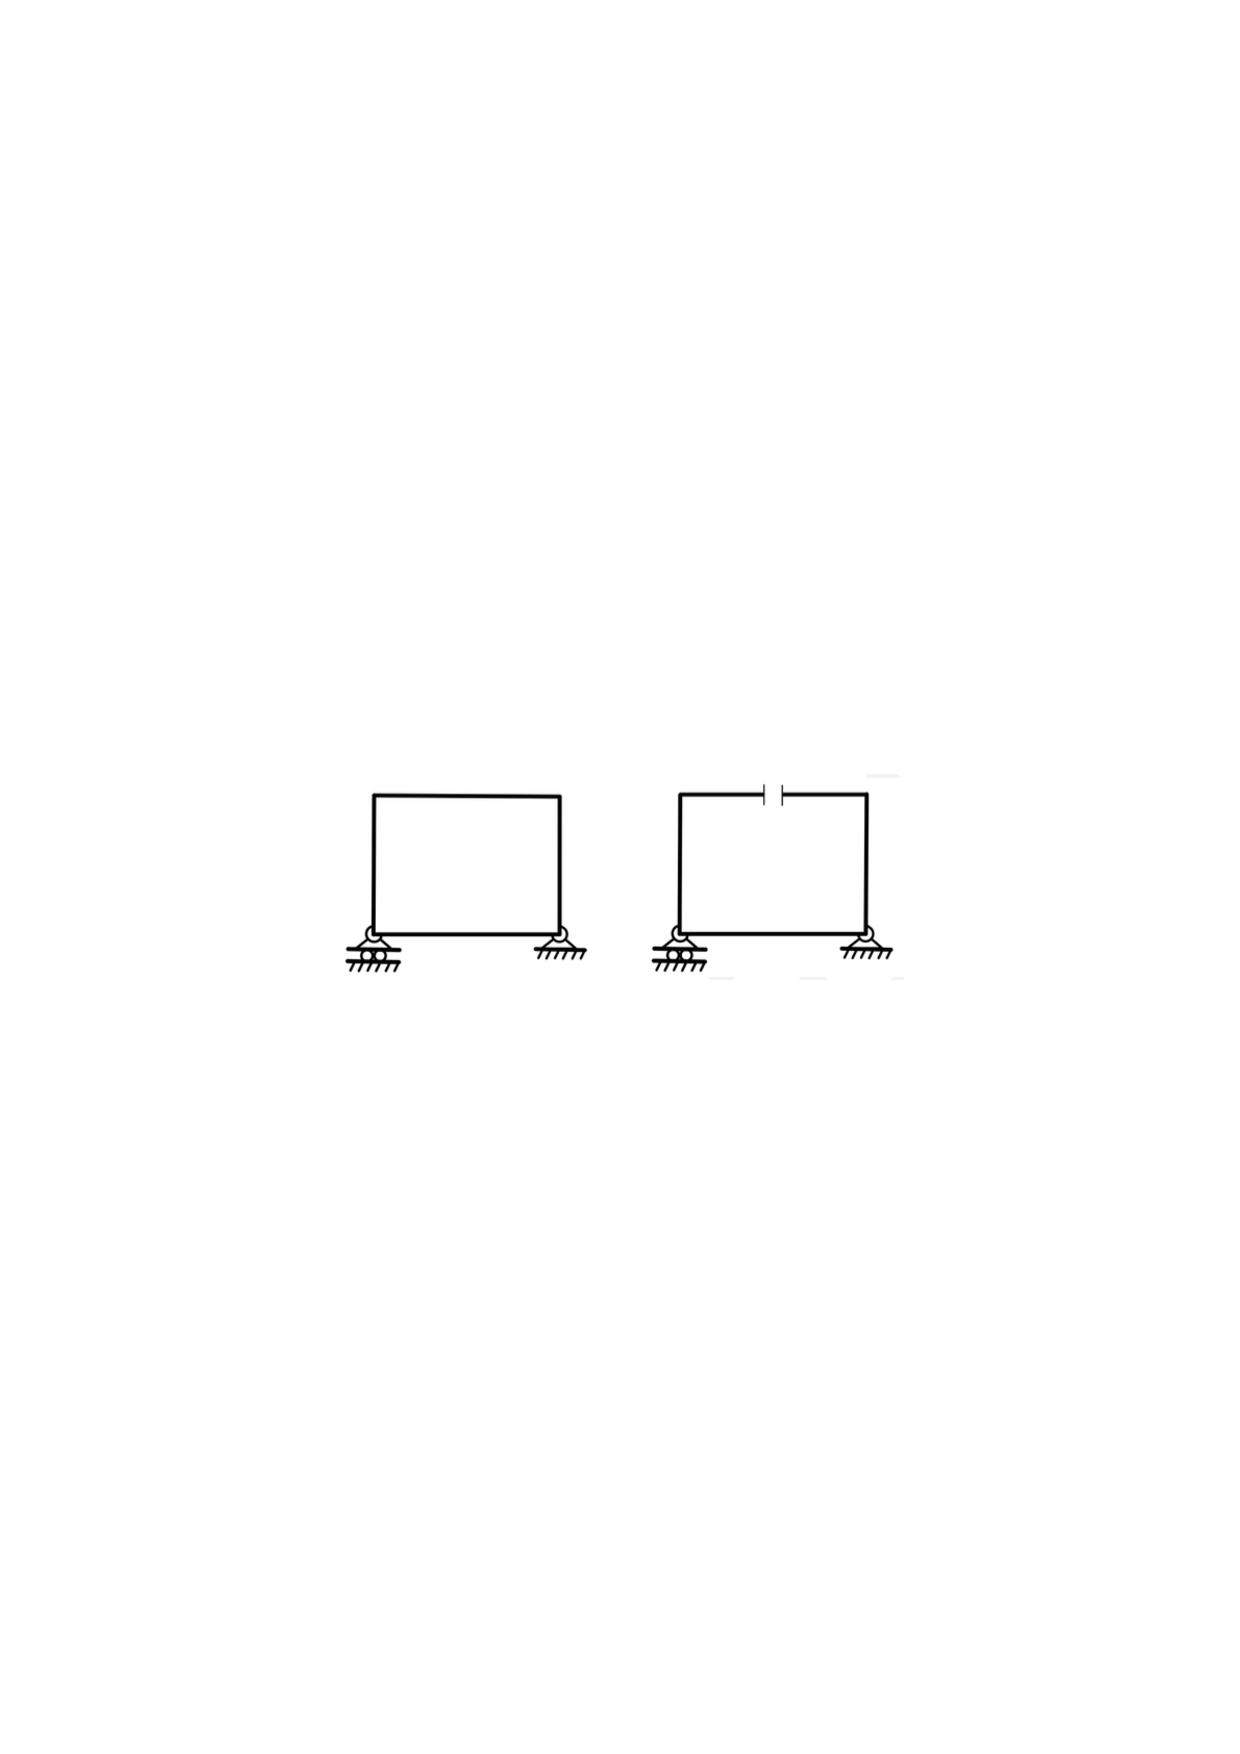
\includegraphics[scale=0.75]{cin_apertifinti.pdf}
		\caption{Portale rettangolare (schema ripreso nel
			Vol.~II per il caso deformabile): maglia chiusa
			(sinistra, $\nu = -3$) e maglia aperta con
			taglio completo nella traversa superiore
			(destra, $\nu = 0$). Il taglio rimuove
			esattamente $3(p-1) = 3$ gradi di iperstaticità.}
		\label{fig:portale_biconnesso}
	\end{figure}
	
	\textbf{Pannello sinistro: maglia chiusa.}
	\begin{svolgimento}
		La struttura è composta da quattro elementi (due
		colonne e due traversi) con nodi rigidi ai quattro
		angoli. Ciascun nodo collega due elementi con
		un incastro interno: molteplicità $3(2-1) = 3$
		per nodo, quattro nodi, $4 \times 3 = 12$ equazioni
		di vincolo interne. I vincoli al suolo aggiungono
		$2 + 1 = 3$ equazioni scalari (cerniera in $A$
		e carrello in $B$). In totale:
		\[
		n_e = 4,\quad n = 12,\quad m = 12 + 3 = 15,
		\quad \nu = 12 - 15 = -3.
		\]
		Il sistema è \textit{iperstatico} di grado~3.
		Tre equazioni in eccesso corrispondono alle tre
		condizioni di chiusura geometrica della maglia:
		non è possibile assegnare liberamente gli
		spostamenti relativi nella sezione di taglio
		senza violare la continuità dell'anello.
	\end{svolgimento}
	
	\textbf{Pannello destro: taglio completo.}
	\begin{svolgimento}
		Il taglio introduce tre svincoli simultanei nella
		traversa superiore, rilasciando tutte le condizioni
		di continuità in quella sezione: la maglia si apre
		completamente e $\nu$ aumenta di~3.
		\[
		\nu = -3 + 3 = 0.
		\]
		La struttura aperta risultante è un unico corpo
		rigido equivalente --- le due colonne e i due
		semitravetti sono tutti collegati da nodi rigidi
		--- vincolato al suolo da cerniera in $A$ e
		carrello in $B$. Il sistema	è \textit{isostatico}.
	\end{svolgimento}
\end{esempio}

%--------------------------------------------------------------
\begin{esempio}[Telaio a tre piani: pluriconnesso e tagli
	progressivi]
	\label{ex:telaio_pluriconnesso}
	Si consideri il telaio della
	\FIGref{fig:telaio_pluriconnesso}: due colonne
	incastrate alla base, tre traversi con nodi rigidi
	ai sei angoli. La struttura presenta tre maglie
	chiuse, una per piano, formate ciascuna dai due
	tratti di colonna e dal traverso corrispondente.
	I pannelli centrale e destro mostrano la progressiva
	apertura delle maglie con tagli completi nei traversi.
	
	\begin{figure}[ht]
		\centering
		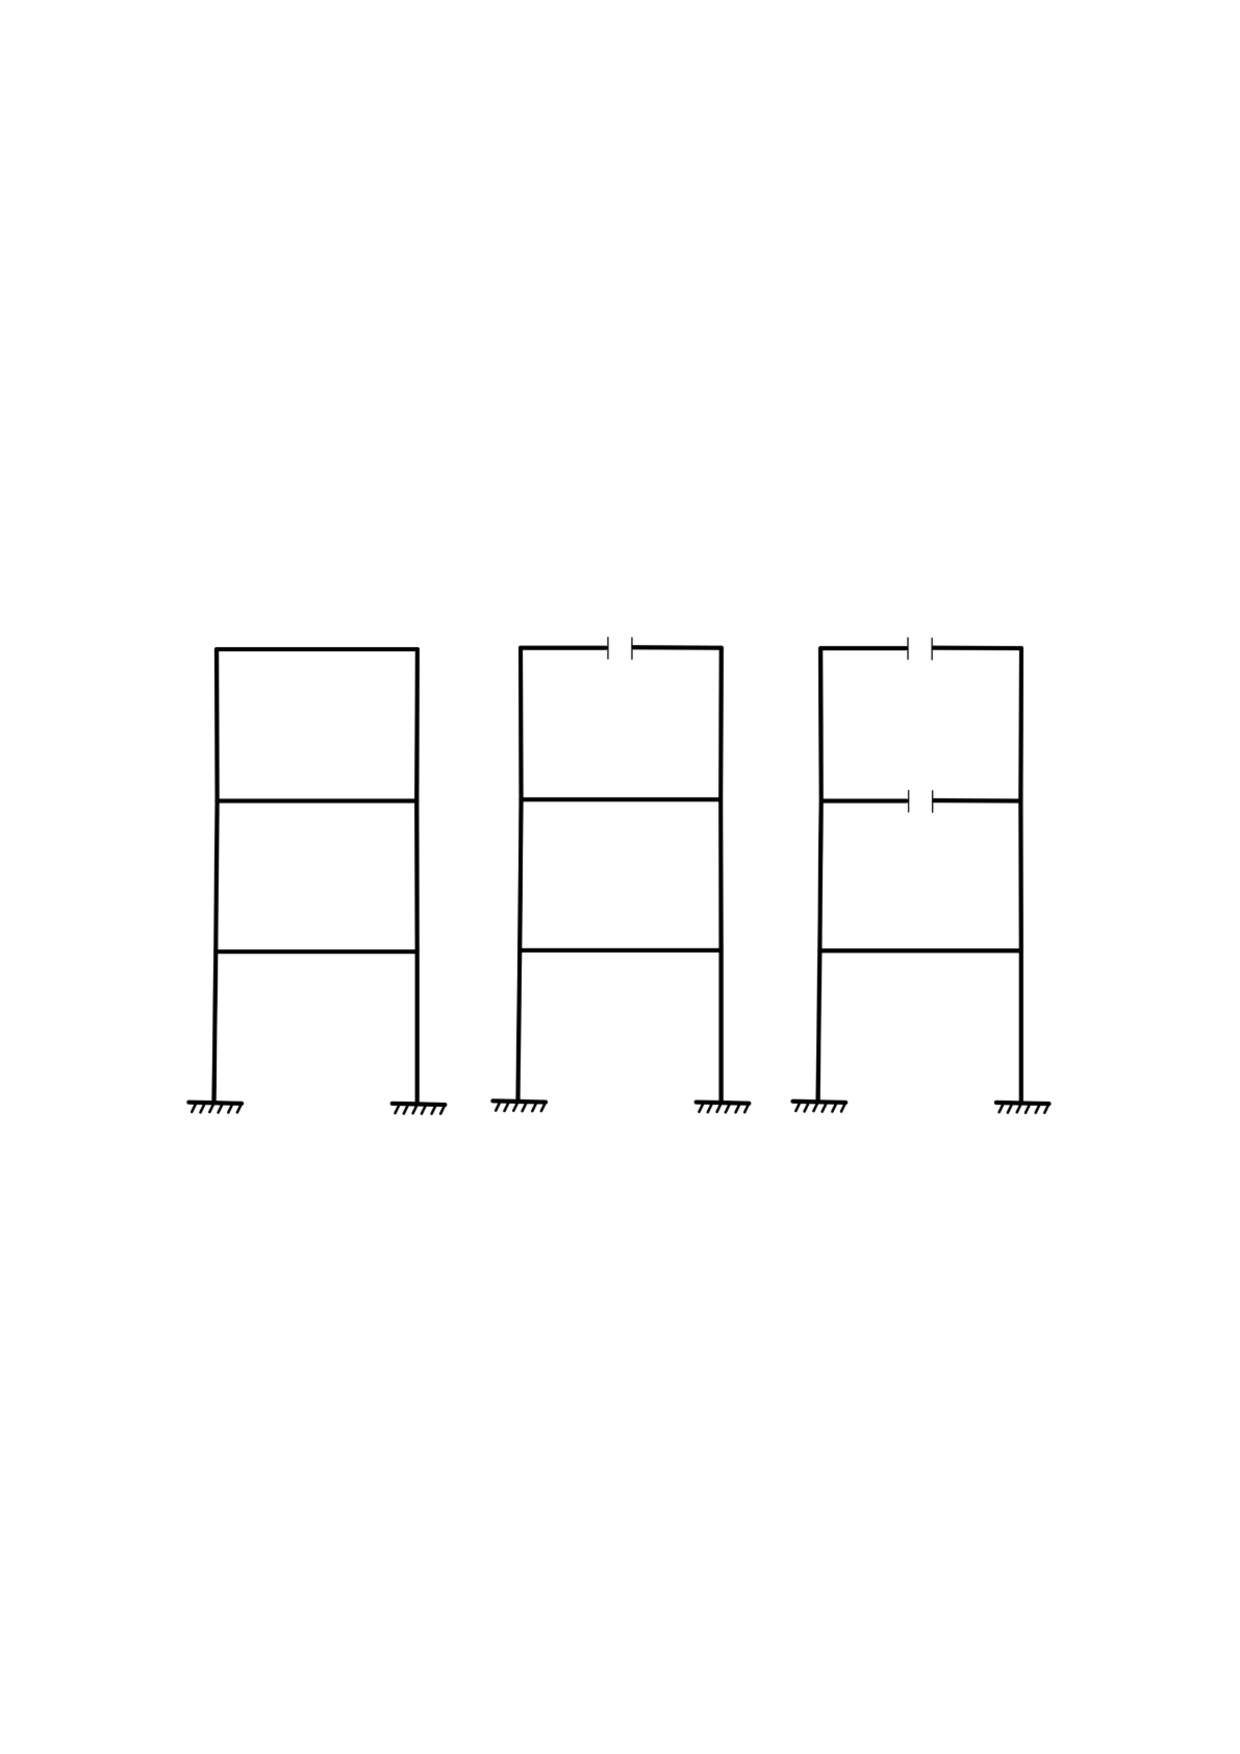
\includegraphics[scale=0.75]{cin_multipiano.pdf}
		\caption{Telaio a tre piani (schema ripreso nel
			Vol.~II per il caso deformabile): tre
			configurazioni con gradi di iperstaticità
			decrescenti. Da sinistra: tre maglie chiuse
			($\nu = -9$); taglio completo nella traversa
			superiore, due maglie chiuse ($\nu = -6$);
			tagli nelle traversi superiore e intermedia,
			una maglia chiusa ($\nu = -3$). Un terzo
			taglio aprirebbe l'ultima maglia ($\nu = 0$).}
		\label{fig:telaio_pluriconnesso}
	\end{figure}
	
	\textbf{Pannello sinistro: tre maglie chiuse.}
	\begin{svolgimento}
		La struttura ha nove elementi: sei tratti di
		colonna ($AC$, $CE$, $EG$, $BD$, $DF$, $FH$)
		e tre traversi ($CD$, $EF$, $GH$), con $n = 27$.
		I nodi ai quattro angoli di piano ($C$, $D$,
		$E$, $F$) collegano tre elementi con incastro
		interno: molteplicità $3(3-1) = 6$ per nodo.
		I nodi in sommità ($G$, $H$) collegano due
		elementi: molteplicità $3(2-1) = 3$ per nodo.
		I due incastri alla base aggiungono $2 \times 3 = 6$
		equazioni scalari. In totale:
		\[
		n = 27, \quad
		m = 4 \times 6 + 2 \times 3 + 6 = 36,
		\quad \nu = 27 - 36 = -9.
		\]
		Il sistema è \textbf{iperstatico di grado~9}:
		le nove equazioni in eccesso corrispondono alle
		tre condizioni di chiusura geometrica di ciascuna
		delle tre maglie.
	\end{svolgimento}
	
	\textbf{Pannelli centrale e destro: tagli progressivi.}
	\begin{svolgimento}
		Ogni taglio completo in un traverso apre la
		maglia corrispondente e aumenta $\nu$ di~3:
		\begin{itemize}[nosep]
			\item taglio nella traversa superiore:
			$\nu = -9 + 3 = -6$, due maglie chiuse;
			\item taglio anche nella traversa intermedia:
			$\nu = -6 + 3 = -3$, una maglia chiusa;
			\item un terzo taglio nella traversa inferiore:
			$\nu = -3 + 3 = 0$, nessuna maglia chiusa;
			il sistema è \textit{isostatico}.
		\end{itemize}
	\end{svolgimento}
	
	\begin{oss}
		La progressione mostra come interventi topologici
		mirati --- i tagli completi --- controllino
		sistematicamente l'iperstaticità del telaio.
		Un telaio rettangolare a $n_p$ piani e $n_c$
		campate ha $n_p \times n_c$ maglie chiuse e
		iperstaticità $3\,n_p\,n_c$, prima di considerare
		i vincoli esterni.
	\end{oss}
\end{esempio}



%----------------------------------------------------------------------------------------------------------------------------
\section{Isostaticità globale e locale}
\label{sec:globale_locale}
%----------------------------------------------------------------------------------------------------------------------------

Nei sistemi a più corpi è utile distinguere due livelli di
analisi: quello \emph{globale}, relativo al comportamento del
sistema nel suo insieme nei confronti del suolo, e quello
\emph{locale}, relativo alla distribuzione degli spostamenti
e delle forze tra i singoli corpi all'interno del sistema.
I vincoli esterni --- tra corpi e suolo --- governano il
livello globale; i vincoli interni --- tra corpi distinti ---
governano il livello locale.

%----------------------------------------------------------------------------------------------------------------------------
\subsection{Definizioni e decomposizione di \texorpdfstring{$\nu$}{ν}}
\label{sec:iso_globale_locale}
%----------------------------------------------------------------------------------------------------------------------------

\paragraph{Conteggio globale.}\index{conteggio dei gradi di libertà!globale}
Si considerino i soli vincoli esterni, trattando l'intero
sistema come un unico corpo rigido equivalente. Il numero di
vincoli scalari esterni è $m_{\rm est}$; il numero nominale
di gradi di libertà globali è
\begin{equation}\label{eq:nu_glob}
	\nu_{\rm glob} = 3 - m_{\rm est}.
\end{equation}
Il sistema è \emph{globalmente isostatico}\index{isostaticita@isostaticità!globale|textbf} se $\nu_{\rm glob}
= 0$ e i vincoli esterni sono geometricamente non degeneri.
In tal caso, dal lato statico, le reazioni esterne sono
univocamente determinate dall'equilibrio del sistema
considerato come un corpo unico, indipendentemente da come
le forze si distribuiscono internamente. Dal lato cinematico,
eventuali cedimenti dei soli vincoli esterni producono un
moto rigido d'insieme della struttura: tutti i corpi si
spostano solidalmente, senza deformazioni relative tra loro.

\paragraph{Conteggio locale.}\index{conteggio dei gradi di libertà!locale}
Si considerino i soli vincoli interni, fissando il sistema
rispetto al suolo. Il numero di vincoli scalari interni è
$m_{\rm int}$; i gradi di libertà interni --- quelli che
descrivono i moti relativi tra i corpi, al netto dei moti
rigidi d'insieme --- sono $3(n_c - 1)$. Il numero nominale
di gradi di libertà locali è quindi
\begin{equation}\label{eq:nu_loc}
	\nu_{\rm loc} = 3(n_c - 1) - m_{\rm int}.
\end{equation}
Il sistema è \emph{localmente isostatico}\index{isostaticita@isostaticità!locale|textbf} se $\nu_{\rm loc}
= 0$ e i vincoli interni sono geometricamente non degeneri.
In tal caso, dal lato statico, le forze interne tra i corpi
sono univocamente determinate dall'equilibrio dei singoli
corpi liberi, una volta note le reazioni esterne. Dal lato
cinematico, eventuali distorsioni ai vincoli di continuità
e cedimenti dei vincoli interni di collegamento tra corpi
--- cedimenti relativi assegnati in una cerniera interna,
scorrimento relativo lungo un pendolo interno, e così via
--- sono compatibili con spostamenti che si riducono a moti
rigidi di ciascun corpo: non esistono meccanismi interni
che coinvolgano deformazioni relative non prescritte.

\paragraph{Decomposizione di $\nu$.}
Poiché $m = m_{\rm est} + m_{\rm int}$, sommando
\eqref{eq:nu_glob} e \eqref{eq:nu_loc} si ottiene:
\begin{equation}\label{eq:nu_decomp}
	\nu_{\rm glob} + \nu_{\rm loc}
	= 3 - m_{\rm est} + 3(n_c-1) - m_{\rm int}
	= 3n_c - m = \nu.
\end{equation}
Il numero nominale complessivo $\nu$ si decompone
esattamente in contributo globale e contributo locale.
I due contributi sono indipendenti nel conteggio nominale,
ma possono interferire geometricamente: un sistema con
$\nu_{\rm glob} = \nu_{\rm loc} = 0$ può essere comunque
degenere se la disposizione dei vincoli produce perdite di
rango globale o locale.

\begin{oss}[Isostaticità completa]
	Il sistema è \emph{completamente isostatico}\index{isostaticita@isostaticità!completa|textbf} quando
	$\nu_{\rm glob} = \nu_{\rm loc} = 0$ e tutti i vincoli
	--- esterni e interni --- sono geometricamente non
	degeneri: in tal caso $g_\ell = g_{\mathscr{i}} = 0$
	(\TABref{tab:classificazione} del
	\CAPref{cap:problemi_cin_stat_SCR}). Dal lato statico,
	sia le reazioni esterne sia le forze interne sono
	univocamente determinate dall'equilibrio. Dal lato
	cinematico, la configurazione del sistema è
	univocamente determinata da cedimenti e distorsioni
	assegnati: non esistono né moti rigidi d'insieme
	né meccanismi interni.
\end{oss}

%----------------------------------------------------------------------------------------------------------------------------
\subsection{Casi possibili e loro significato}
\label{sec:casi_globale_locale}
%----------------------------------------------------------------------------------------------------------------------------

La combinazione dei due livelli produce quattro casi
significativi, illustrati nella \TABref{tab:globale_locale}.

\begin{table}[ht]
	\centering
	\renewcommand{\arraystretch}{1.8}
	\small
	\begin{tabular}{ccp{8cm}}
		\toprule
		Globale & Locale & Significato \\
		\midrule
		Isostatico & Isostatico
		& Sistema completamente determinato: reazioni esterne
		e forze interne univocamente determinate. \\
		Isostatico & Labile
		& Le reazioni esterne sono determinate, ma esistono
		meccanismi interni: i corpi possono muoversi
		relativamente l'uno all'altro pur restando in
		equilibrio globale. Il sistema complessivo è labile
		($g_\ell = |\nu_{\rm loc}| > 0$). \\
		Isostatico & Iperstatico
		& Le reazioni esterne sono determinate, ma le forze
		interne sono in parte indeterminate: i vincoli interni
		sono ridondanti e ammettono stati di autoequilibrio
		interno. Il sistema complessivo è iperstatico
		($g_{\mathscr{i}} = |\nu_{\rm loc}| > 0$). \\
		Labile o Iperstatico & qualsiasi
		& Il sistema non è in equilibrio globale per carichi
		generici (labile) oppure le reazioni esterne sono
		indeterminate (iperstatico esterno). \\
		\bottomrule
	\end{tabular}
	\caption{Combinazioni di isostaticità globale e locale
		per un sistema di corpi rigidi piani.
		La condizione $\nu_{\rm glob} = 0$ è necessaria
		per l'isostaticità globale; la condizione
		$\nu_{\rm loc} = 0$ è necessaria per quella locale.
		Entrambe le condizioni sono necessarie ma non
		sufficienti in presenza di degenerazioni geometriche.}
	\label{tab:globale_locale}
\end{table}

\begin{esempio}[Sistema globalmente isostatico e localmente labile]
	\label{ex:glob_iso_loc_lab}
	Si considerino due corpi $\mathcal{C}_1$ e $\mathcal{C}_2$
	($n_c = 2$) collegati da un pendolo interno in $C$
	($m_{\rm int} = 1$) e vincolati al suolo da una cerniera
	in $A$ su $\mathcal{C}_1$ e un carrello in $B$ su
	$\mathcal{C}_2$ ($m_{\rm est} = 2 + 1 = 3$).
	
	\smallskip
	\noindent\textit{Livello globale.}
	I tre vincoli esterni ($m_{\rm est} = 3$) danno
	$\nu_{\rm glob} = 3 - 3 = 0$: nella configurazione
	regolare il sistema è globalmente isostatico e le tre
	reazioni esterne $X_A$, $Y_A$, $R_B$ sono determinate
	univocamente dall'equilibrio del sistema considerato come
	corpo unico.
	
	\smallskip
	\noindent\textit{Livello locale.}
	Il solo vincolo interno ($m_{\rm int} = 1$) dà
	$\nu_{\rm loc} = 3(2-1) - 1 = 2$: il sistema è
	localmente labile di grado~2. Le due componenti dello
	spostamento relativo tra i corpi nella direzione
	trasversale al pendolo e la rotazione relativa sono
	libere; la sola componente assiale al pendolo è vincolata.
	
	\smallskip
	\noindent\textit{Classificazione complessiva.}
	$\nu = \nu_{\rm glob} + \nu_{\rm loc} = 0 + 2 = 2$:
	il sistema è labile di grado~2 nonostante l'isostaticità
	globale. Le reazioni esterne sono determinate ma i due
	corpi non sono vincolati a muoversi come un unico
	solido rigido.
\end{esempio}

\begin{esempio}[Sistema globalmente isostatico e localmente labile]
	\label{ex:glob_iso_loc_iper}
	Si modifichi l'esempio precedente sostituendo il pendolo
	interno con una cerniera interna in $C$
	($m_{\rm int} = 2$), mantenendo invariati i vincoli
	esterni ($m_{\rm est} = 3$). Totale: $m = 5$,
	$\nu = 6 - 5 = 1$.
	
	\smallskip
	\noindent\textit{Livello globale.}
	Invariato rispetto all'esempio precedente:
	$\nu_{\rm glob} = 3 - 3 = 0$. Dal lato statico
	le reazioni esterne $X_A$, $Y_A$, $R_B$ sono
	univocamente determinate dall'equilibrio del
	sistema considerato come corpo unico. Dal lato
	cinematico, eventuali cedimenti dei vincoli
	esterni producono un moto rigido d'insieme.
	
	\smallskip
	\noindent\textit{Livello locale.}
	$\nu_{\rm loc} = 3(2-1) - 2 = 1$: il sistema è
	localmente labile di grado~1. Dal lato cinematico,
	la rotazione relativa tra i due corpi attorno a
	$C$ è libera: la cerniera impone l'uguaglianza
	degli spostamenti in $C$ ma non quella delle
	rotazioni, lasciando libero un grado di libertà
	relativo. Dal lato statico, le due componenti
	della forza interna alla cerniera sono determinate
	dall'equilibrio dei due corpi liberi, ma non esiste
	un'equazione cinematica di vincolo duale al momento
	flettente relativo: la cerniera non trasmette
	momento, e questa grandezza è identicamente nulla
	per costruzione.
	
	\smallskip
	\noindent\textit{Raggiungimento dell'isostaticità
		completa.}
	Per portare $\nu_{\rm loc}$ a zero occorre
	aggiungere un vincolo scalare interno o esterno.
	Due strade sono possibili:
	
	\begin{itemize}[nosep]
		\item \emph{Intervento interno}: si aggiunge
		un bipendolo in $C$ ($m_{\rm int} = 2 + 1 = 3$,
		$\nu_{\rm loc} = 3 - 3 = 0$). Il bipendolo
		ripristina la condizione di uguale rotazione
		in $C$: i due corpi si fondono in un unico
		corpo equivalente e il sistema si riduce a
		una trave appoggiata.
		
		\item \emph{Intervento esterno}: si aggiunge
		un pendolo esterno in $B$ ($m_{\rm est} = 3
		+ 1 = 4$, $\nu_{\rm glob} = 3 - 4 = -1$,
		$\nu_{\rm loc} = 1$, $\nu = 0$). Il pendolo
		blocca il grado di libertà relativo residuo
		agendo dall'esterno, senza modificare la
		struttura interna.
	\end{itemize}
	
	\begin{oss}
		I due interventi che portano a $\nu = 0$
		illustrano una distinzione importante: il grado
		di libertà locale residuo può essere eliminato
		agendo sui vincoli interni oppure su quelli
		esterni. Nel primo caso l'isostaticità è
		completa: $\nu_{\rm glob} = \nu_{\rm loc} = 0$.
		Nel secondo caso si ha $\nu_{\rm glob} = -1$ e
		$\nu_{\rm loc} = 1$: i due contributi si
		compensano ma la struttura interna è diversa ---
		i due corpi restano distinti con un grado di
		libertà relativo bloccato dall'esterno.
		In sintesi: il primo intervento agisce su
		$\nu_{\rm loc}$, il secondo su $\nu_{\rm glob}$,
		pur producendo entrambi $\nu = 0$. La
		decomposizione globale/locale è lo strumento
		che rende visibile questa differenza.
	\end{oss}
\end{esempio}

\begin{oss}[Limite del conteggio globale/locale]
	La decomposizione~\eqref{eq:nu_decomp} si basa sul
	conteggio delle molteplicità e vale come condizione
	necessaria. Non è detto che un sistema con
	$\nu_{\rm glob} = 0$ sia effettivamente globalmente
	isostatico: se i vincoli esterni sono geometricamente
	degeneri --- ad esempio paralleli o concorrenti ---
	la matrice di equilibrio globale perde rango e il
	sistema è globalmente labile-iperstatico pur con
	$\nu_{\rm glob} = 0$. I criteri geometrici per
	identificare queste degenerazioni sono sviluppati
	nelle \PARref{sec:catalogo}--\ref{sec:ispezione}.
\end{oss}



%----------------------------------------------------------------------------------------------------------------------------
\section{Catalogo delle sottostrutture elementari}
\label{sec:catalogo}
%----------------------------------------------------------------------------------------------------------------------------

La classificazione di un sistema complesso può spesso essere
ricondotta al riconoscimento di sottostrutture elementari\index{sottostruttura elementare} note.
In questa sezione si presenta un catalogo delle sottostrutture
più frequenti, organizzato per numero di corpi, con i casi
regolari e degeneri affiancati. La conoscenza di questi elementi
consente di classificare sistemi più complessi per
\emph{decomposizione}, senza costruire esplicitamente $\bm{A}$.

Per ogni sottostruttura si indicano: il numero di corpi $n_c$,
il numero di vincoli scalari $m$, il numero nominale di gradi
di libertà $\nu = 3n_c - m$, e la classificazione effettiva
con le condizioni geometriche che la determinano.

%----------------------------------------------------------------------------------------------------------------------------
\subsection{Un corpo: mensola e trave appoggiata}
\label{sec:catalogo_1corpo}
%----------------------------------------------------------------------------------------------------------------------------

Il caso di un singolo corpo rigido piano ($n_c = 1$, $n = 3$)
è completamente determinato dai tre parametri $(u(O), v(O), \vartheta)$.
Le due sottostrutture di riferimento sono la mensola e la trave
appoggiata.

\paragraph{Mensola.}\index{mensola|textbf}
Un incastro al suolo in $A$ fornisce $m = 3$ vincoli scalari,
dunque $\nu = 0$. Poiché l'incastro blocca simultaneamente le
due traslazioni e la rotazione del punto $A$, la matrice
$\bm{A}$ è l'identità $3 \times 3$: il sistema è
\textit{isostatico} in qualsiasi configurazione. Le tre reazioni $X_A$, $Y_A$, $\mu_A$ sono 
indipendenti e sufficienti a garantire l'equilibrio 
per qualsiasi sistema di forze applicato.

\begin{figure}[ht]
	\centering
	%\includegraphics[width=0.5\textwidth]{fig_catalogo_mensola}
	\caption{Mensola: incastro in $A$, $m=3$, $\nu=0$, isostatica.
		Le tre reazioni $X_A$, $Y_A$, $\mu_A$ sono indipendenti
		e sufficienti a equilibrare qualsiasi sistema di forze
		applicato.}
	\label{fig:catalogo_mensola}
\end{figure}

\paragraph{Trave semplicemente appoggiata.}\index{trave!semplicemente appoggiata|textbf}
Una cerniera in $A$ (2 vincoli) e un carrello in $B$ (1 vincolo)
forniscono $m = 3$ vincoli scalari, $\nu = 0$.

\smallskip
\noindent\textit{Caso regolare.}
Se la linea d'azione del carrello in $B$ non passa per $A$,
i tre vincoli sono geometricamente indipendenti:
$\rg(\bm{A}) = 3$ e il sistema è \textit{isostatico}
(\FIGref{fig:catalogo_trave_carrello}\,a).
Il centro di rotazione assoluto è fissato in $A$ dalla
cerniera; il carrello impone che il centro giaccia su una
retta per $B$ nella direzione del proprio asse --- retta
che, per ipotesi, non passa per $A$ --- determinando
univocamente $\vartheta = 0$ e quindi la configurazione.
Dal lato statico, le due componenti della reazione
in $A$ bilanciano qualsiasi forza risultante applicata
al corpo, mentre la reazione in $B$ --- essendo la sua
linea d'azione non passante per $A$ --- consente di
soddisfare l'equilibrio dei momenti rispetto ad $A$.

\smallskip
\noindent\textit{Caso degenere.}
Se la linea d'azione del carrello in $B$ passa per $A$,
le equazioni della cerniera e del carrello si riducono
a due condizioni sullo spostamento di $A$: il sistema è
\textit{labile-iperstatico} con $g_\ell = g_{\mathscr{i}} = 1$
(\FIGref{fig:catalogo_trave_carrello}\,b).
Il meccanismo è la rotazione attorno ad $A$: sia la
cerniera ($\ub(A) = \zerovb$) sia il carrello
($\ub(B) \cdot \ab = 0$ verificata per qualsiasi rotazione
attorno ad $A$, poiché la linea d'azione passa per $A$)
sono soddisfatti. Dal lato statico, la reazione del carrello in $B$
ha linea d'azione passante per $A$: il suo momento
rispetto ad $A$ è nullo, come quello della reazione
della cerniera in $A$. Nessuna combinazione delle
due reazioni può equilibrare una coppia applicata
al corpo: esiste una forza --- la coppia --- che
i vincoli non riescono a bilanciare. Dualmente,
esiste uno stato di autoequilibrio: una forza nella
direzione dell'asse del carrello, applicata in $B$,
è equilibrata dalla reazione della cerniera in $A$
senza produrre momento risultante, poiché entrambe
le linee d'azione passano per $A$.


\begin{figure}[!ht]
	\centering
	\begin{tikzpicture}[>=Stealth, line width=0.8pt]
		
		\def\L{4.0}
		
		% ============================================================
		% PANNELLO (a) — caso regolare
		% ============================================================
		\begin{scope}[xshift=0cm]
			
			% trave
			\draw[line width=1.5pt] (0,0) -- (\L,0);
			
			% --- cerniera in A (cerniera al suolo) ---
			\draw[thick] (0,0) -- (-0.22,-0.38) -- (0.22,-0.38) -- cycle;
			\draw[thick] (-0.32,-0.38) -- (0.32,-0.38);
			\foreach \x in {-0.24,-0.12,0,0.12,0.24}{
				\draw[thin] (\x,-0.38) -- (\x-0.10,-0.52);
			}
			\node[circle, fill=white, draw=black, inner sep=0pt,
			minimum size=5pt, line width=0.8pt] at (0,0) {};
			
			% --- carrello in B (asse verticale, sotto la trave) ---
			\draw[thick] (\L,0) -- (\L-0.22,-0.38)
			-- (\L+0.22,-0.38) -- cycle;
			\draw[thick] (\L-0.15,-0.44) circle (0.07);
			\draw[thick] (\L+0.15,-0.44) circle (0.07);
			\draw[thick] (\L-0.32,-0.54) -- (\L+0.32,-0.54);
			\foreach \x in {-0.24,-0.12,0,0.12,0.24}{
				\draw[thin] (\L+\x,-0.54) -- (\L+\x-0.10,-0.68);
			}
			\node[circle, fill=white, draw=black, inner sep=0pt,
			minimum size=5pt, line width=0.8pt] at (\L,0) {};
			
			% --- etichette dei nodi ---
			\node[above left,  font=\scriptsize] at (0,0)  {$A$};
			\node[above right, font=\scriptsize] at (\L,0) {$B$};
			
			% --- didascalia del pannello ---
			\node[font=\scriptsize] at (\L/2,-1.20)
			{(a) caso regolare, $\rg(\bm{A})=3$};
			
		\end{scope}
		
		
		% ============================================================
		% PANNELLO (b) — caso degenere (carrello con asse orizzontale)
		% ============================================================
		\begin{scope}[xshift=6.5cm]
			
			\def\thetadeg{15}   % ampiezza dell'angolo di rotazione, in gradi
			
			
			% --- meccanismo (cinematica infinitesima): rotazione theta attorno ad A ---
			% B' è sotto B alla distanza theta*L (linearizzato), sulla verticale di B
			\def\dB{1.0}   % ampiezza grafica del cedimento verticale di B (= theta*L)
			
			% trave deformata: A fisso, B' = B - dB * \ab_y
			\draw[gray!55, line width=1.2pt] (0,0) -- (\L,-\dB);
			
			% etichetta B'
			\node[gray!70,  right, font=\scriptsize] at (\L,-\dB) {$B'$};
			
			% freccia dello spostamento u(B), dal B originale verso B' (verticale)
			\draw[->, gray!70, thick] (\L,0) -- (\L,-\dB);
			\node[gray!70, right, font=\scriptsize] at (\L,-\dB/2) {$q$};
			
			% --- trave (configurazione iniziale) ---
			\draw[line width=1.5pt] (0,0) -- (\L,0);
			
			% --- cerniera in A (cerniera al suolo) ---
			\draw[thick] (0,0) -- (-0.22,-0.38) -- (0.22,-0.38) -- cycle;
			\draw[thick] (-0.32,-0.38) -- (0.32,-0.38);
			\foreach \x in {-0.24,-0.12,0,0.12,0.24}{
				\draw[thin] (\x,-0.38) -- (\x-0.10,-0.52);
			}
			\node[circle, fill=white, draw=black, inner sep=0pt,
			minimum size=5pt, line width=0.8pt] at (0,0) {};
			
			% --- carrello in B con asse ORIZZONTALE (a muro, a destra) ---
			\draw[thick] (\L,0) -- (\L+0.38,-0.22)
			-- (\L+0.38, 0.22) -- cycle;
			\draw[thick] (\L+0.44,-0.15) circle (0.07);
			\draw[thick] (\L+0.44, 0.15) circle (0.07);
			\draw[thick] (\L+0.54,-0.32) -- (\L+0.54, 0.32);
			\foreach \y in {-0.24,-0.12,0,0.12,0.24}{
				\draw[thin] (\L+0.54,\y) -- (\L+0.68,\y-0.10);
			}
			\node[circle, fill=white, draw=black, inner sep=0pt,
			minimum size=5pt, line width=0.8pt] at (\L,0) {};
			
			% --- linea d'azione di R_B (tratteggiata lungo AB) ---
			\draw[dashed, thin, gray!70] (-0.5,0) -- (\L+0.5,0);
			\node[font=\scriptsize, gray!80] at (\L/2,0.30)
			{linea d'azione di $R_B$};
			
			% --- etichette dei nodi (in primo piano) ---
			\node[above left,  font=\scriptsize] at (0,0)   {$A$};
			\node[above,       font=\scriptsize] at (\L,0.05) {$B$};
			
			% --- didascalia del pannello ---
			\node[font=\scriptsize] at (\L/2,-1.20)
			{(b) caso degenere, $g_\ell = g_{\mathscr{i}} = 1$};
			
		\end{scope}
		
	\end{tikzpicture}
	\caption{Trave appoggiata: \emph{(a)}~caso regolare, $\rg(\bm{A})=3$ (isostatico); \emph{(b)}~caso	degenere, $g_\ell = g_{\mathscr{i}} = 1$. In (b) la	linea d'azione del carrello (tratteggio grigio)	coincide con la retta $AB$; il meccanismo è	rappresentato dalla configurazione deformata	(grigio) e dal parametro lagrangiano $q$.}
	\label{fig:catalogo_trave_carrello}
	\label{fig:catalogo_trave_carrello}
\end{figure}


\paragraph{Trave con glifo.}\index{trave!con glifo|textbf}
Una variante si ottiene sostituendo la cerniera in $A$
con un \emph{glifo} di asse $\ab_g$ (2 vincoli scalari).
La trave è quindi vincolata da un glifo in $A$ (2 vincoli)
e un carrello in $B$ di asse $\ab_c$ (1 vincolo):
$m = 2 + 1 = 3$, $\nu = 0$.

\smallskip
\noindent\textit{Caso regolare.}
Se gli assi $\ab_g$ e $\ab_c$ non sono paralleli, i tre
vincoli sono geometricamente indipendenti:
$\rg(\bm{A}) = 3$ e il sistema è \textit{isostatico}
(\FIGref{fig:catalogo_trave_glifo}\,a).
Il glifo impone $\vartheta = 0$ (rotazione bloccata) e una
condizione di traslazione perpendicolare ad $\ab_g$;
il carrello impone una seconda condizione di traslazione
perpendicolare ad $\ab_c$. Quando $\ab_g \not\parallel \ab_c$
le due condizioni sono indipendenti e fissano univocamente
lo spostamento del corpo.

\smallskip
\noindent\textit{Caso degenere.}
Se gli assi $\ab_g$ e $\ab_c$ sono paralleli, le due
condizioni di traslazione coincidono: $\rg(\bm{A}) = 2$ e
il sistema è \textit{labile-iperstatico} con
$g_\ell = g_{\mathscr{i}} = 1$
(\FIGref{fig:catalogo_trave_glifo}\,b).
Il meccanismo è la traslazione del corpo nella direzione
comune dei due assi: la rotazione resta bloccata dal glifo,
ma lo spostamento parallelo agli assi non è impedito da
alcun vincolo. Dal lato statico, esiste uno stato di
autoequilibrio: una coppia di forze uguali e opposte,
perpendicolari agli assi e applicate in $A$ e $B$, è
equilibrata da una reazione di coppia nel glifo, poiché
entrambi i vincoli possono sviluppare reazioni in quella
direzione.


\begin{figure}[!ht]
	\centering
	\begin{tikzpicture}[>=Stealth, line width=0.8pt]
		
		\def\L{4.0}
		
		% ============================================================
		% PANNELLO (a) — caso regolare (assi non paralleli)
		% ============================================================
		\begin{scope}[xshift=0cm]
			
			% --- trave (orizzontale, in y=0, parte dall'origine) ---
			\draw[line width=1.5pt] (0,0) -- (\L,0);
			
			% --- GLIFO in A: piatti a -45° (orario), agganciato alla
			\begin{scope}[shift={({-0.12*sin(45)}, {-0.12*cos(45)})},
				rotate=-45]
				% piatto inferiore
				\draw[thick] (-0.45,-0.12) -- (0.45,-0.12);
				% piatto superiore
				\draw[thick] (-0.45, 0.12) -- (0.45, 0.12);
				% rotelle (cerchietti tra i piatti)
				\draw[thick] (-0.15, 0) circle (0.10);
				\draw[thick] ( 0.15, 0) circle (0.10);
				% hatching sotto il piatto inferiore (a indicare il suolo)
				\foreach \x in {-0.36,-0.18,0,0.18,0.36}{
					\draw[thin] (\x,-0.12) -- (\x-0.10,-0.26);
				}
			\end{scope}
			
			% --- freccia ed etichetta asse del glifo a_g a +45° ---
			\draw[->, thin, gray!70] (0,0) -- ({0.55*cos(45)}, {0.55*sin(45)});
			\node[gray!80, font=\scriptsize, right] at	({0.55*cos(45)+0.05}, {0.55*sin(45)+0.02}) {$\ab_g$};
			
			% --- CARRELLO in B: asse verticale ---
			\draw[thick] (\L,0) -- (\L-0.22,-0.38)
			-- (\L+0.22,-0.38) -- cycle;
			\draw[thick] (\L-0.15,-0.44) circle (0.07);
			\draw[thick] (\L+0.15,-0.44) circle (0.07);
			\draw[thick] (\L-0.32,-0.54) -- (\L+0.32,-0.54);
			\foreach \x in {-0.24,-0.12,0,0.12,0.24}{
				\draw[thin] (\L+\x,-0.54) -- (\L+\x-0.10,-0.68);
			}
			\node[circle, fill=white, draw=black, inner sep=0pt,
			minimum size=5pt, line width=0.8pt] at (\L,0) {};
			
			% --- freccia ed etichetta asse del carrello a_c verticale ---
			\draw[->, thin, gray!70] (\L,0) -- (\L,0.55);
			\node[gray!80, font=\scriptsize, right] at (\L,0.45) {$\ab_c$};
			
			% --- etichette dei nodi ---
			\node[above ,  font=\scriptsize] at (0,0)  {$A$};
			\node[above right, font=\scriptsize] at (\L,0) {$B$};
			
			% --- didascalia del pannello ---
			\node[font=\scriptsize] at (\L/2,-1.30)
			{(a) caso regolare, $\rg(\bm{A})=3$};
			
		\end{scope}
		
		% ============================================================
		% PANNELLO (b) — caso degenere (assi collineari, opposti)
		% ============================================================
		\begin{scope}[xshift=7.0cm]
			
			\def\q{1.0}
			
			% --- meccanismo: trave traslata di q lungo (-45°) [grigia] ---
			\draw[gray!55, line width=1.2pt] ({\q*cos(45)},{-\q*sin(45)}) -- ({\L+\q*cos(45)},{-\q*sin(45)});
			\node[gray!70, below left,  font=\scriptsize] at({\q*cos(45)},{-\q*sin(45)})  {$A'$};
			\node[gray!70, below right, font=\scriptsize] at ({\L+\q*cos(45)},{-\q*sin(45)}) {$B'$};
			
			% frecce del parametro lagrangiano q in A e in B, lungo -45°
			\draw[->, gray!70, thick] (0,0) --	({\q*cos(45)},{-\q*sin(45)});
			\draw[->, gray!70, thick] (\L,0) --		({\L+\q*cos(45)},{-\q*sin(45)});
			\node[gray!70, font=\scriptsize] at	({0.5*\q*cos(45)+0.10},{-0.5*\q*sin(45)+0.05}) {$q$};
			\node[gray!70, font=\scriptsize] at	({\L+0.5*\q*cos(45)+0.10},{-0.5*\q*sin(45)+0.05}) {$q$};
			
			% --- trave (configurazione iniziale) ---
			\draw[line width=1.5pt] (0,0) -- (\L,0);
			
			% --- GLIFO in A: piatti a -45° (invariato) ---
			\begin{scope}[shift={({-0.12*sin(45)},{-0.12*cos(45)})},
				rotate=-45]
				\draw[thick] (-0.45,-0.12) -- (0.45,-0.12);
				\draw[thick] (-0.45, 0.12) -- (0.45, 0.12);
				\draw[thick] (-0.15, 0) circle (0.10);
				\draw[thick] ( 0.15, 0) circle (0.10);
				\foreach \x in {-0.36,-0.18,0,0.18,0.36}{
					\draw[thin] (\x,-0.12) -- (\x-0.10,-0.26);
				}
			\end{scope}
			% freccia ed etichetta a_g a +45°
			\draw[->, thin, gray!70] (0,0)	-- ({0.55*cos(45)},{0.55*sin(45)});
			\node[gray!80, font=\scriptsize, right] at	({0.55*cos(45)+0.05},{0.55*sin(45)+0.02}) {$\ab_g$};
			
			% --- CARRELLO in B: ruotato così che a_c = -a_g (a +45° + 180° = -135°) ---
			\begin{scope}[shift={(\L,0)}, rotate=135]
				\draw[thick] (0,0) -- (-0.22,-0.38)	-- (0.22,-0.38) -- cycle;
				\draw[thick] (-0.15,-0.44) circle (0.07);
				\draw[thick] ( 0.15,-0.44) circle (0.07);
				\draw[thick] (-0.32,-0.54) -- (0.32,-0.54);
				\foreach \x in {-0.24,-0.12,0,0.12,0.24}{
					\draw[thin] (\x,-0.54) -- (\x-0.10,-0.68);
				}
			\end{scope}
			% perno bianco in B (centro del carrello = punto di attacco)
			\node[circle, fill=white, draw=black, inner sep=0pt,
			minimum size=5pt, line width=0.8pt] at (\L,0) {};
			% freccia ed etichetta a_c a -135° (cioè -a_g, verso basso-sinistra)
			\draw[->, thin, gray!70] (\L,0)
			-- ({\L-0.55*cos(45)},{-0.55*sin(45)});
			\node[gray!80, font=\scriptsize, left] at
			({\L-0.55*cos(45)-0.05},{-0.55*sin(45)-0.02}) {$\ab_c$};
			
			% --- etichette dei nodi ---
			\node[above,  font=\scriptsize] at (0,0)  {$A$};
			\node[above left, font=\scriptsize] at (\L,0) {$B$};
			
			% --- didascalia del pannello ---
			\node[font=\scriptsize] at (\L/2,-1.55)
			{(b) caso degenere, $g_\ell = g_{\mathscr{i}} = 1$};
			
		\end{scope}
	\end{tikzpicture}
	\caption{Trave con glifo in $A$ e carrello in $B$:
		\emph{(a)}~caso regolare con assi $\ab_g$ e $\ab_c$
		non paralleli ($\rg(\bm{A})=3$, isostatico);
		\emph{(b)}~caso degenere con assi $\ab_g$ e $\ab_c$
		collineari ($g_\ell = g_{\mathscr{i}} = 1$). In (b)
		il meccanismo è la traslazione del corpo nella
		direzione ortogonale agli assi, parametrizzata da $q$.}
	\label{fig:catalogo_trave_glifo}
\end{figure}



\begin{oss}[Simmetria dei due casi degeneri]
	I due casi degeneri appena descritti ---
	carrello la cui linea d'azione passa per la
	cerniera, e glifi con assi paralleli --- sono
	manifestazioni dello stesso fenomeno: la perdita
	di indipendenza geometrica tra i vincoli. Nel
	primo caso i vincoli sono \emph{concorrenti}
	nel punto $A$: la reazione del carrello ha
	momento nullo rispetto ad $A$, come quella
	della cerniera, e il sistema non può equilibrare
	una coppia. Nel secondo caso i vincoli sono
	\emph{paralleli}: le due condizioni di
	traslazione coincidono e il sistema non può
	opporsi a una traslazione nella direzione
	comune. Entrambi i pattern si ritrovano, su
	scala più ampia, nei sistemi a più corpi e
	sono discussi sistematicamente nella
	\PARref{sec:ispezione}.
\end{oss}

\paragraph{Trave con tre carrelli.}\index{trave!con tre carrelli|textbf}
Una configurazione che merita attenzione a sé è quella di una
trave con tre carrelli ($m = 3$, $\nu = 0$): il conteggio
suggerisce l'isostaticità, ma la classificazione effettiva
dipende interamente dalla disposizione geometrica degli assi.
Le due degenerazioni tipiche --- assi tutti paralleli e assi
tutti concorrenti in un punto --- sono illustrate
nell'esempio seguente.

\begin{esempio}[Trave con tre carrelli degeneri ---
	assi paralleli e assi concorrenti]
	\label{ex:tre_carrelli_degeneri}
	Si consideri una trave rigida con tre carrelli. Nel
	\textbf{caso~(a)} i tre carrelli hanno tutti asse verticale
	(assi paralleli); nel \textbf{caso~(b)} i tre carrelli hanno
	assi convergenti in un punto proprio $P$ al di sopra della
	trave. In entrambi i casi $m = 3$, $\nu = 0$; si mostra
	che $\rg(\bm{A}) = 2$, quindi $g_\ell = g_{\mathscr{i}} = 1$
	(\FIGref{fig:degen_singolo}).
	
	\begin{svolgimento}
		
		\esottotit{Caso (a): tre carrelli verticali.}
		Con polo $O \equiv A$ la matrice dei vincoli è:
		\[
		\bm{A} =
		\begin{bmatrix}
			0 & 1 & 0 \\
			0 & 1 & \ell/2 \\
			0 & 1 & \ell
		\end{bmatrix}.
		\]
		La prima colonna è identicamente nulla: $u(O)$ non compare in
		nessuna equazione di vincolo. Dunque $\rg(\bm{A}) = 2$ e
		$g_\ell = g_{\mathscr{i}} = 1$.
		
		\smallskip
		\noindent\textit{Meccanismo.}
		Il vettore $\bm{u}_1 = (1, 0, 0)^\top$ soddisfa
		$\bm{A}\bm{u}_1 = \bm{0}$: è una traslazione orizzontale pura.
		Geometricamente, il centro di rotazione assoluto è il punto
		improprio della direzione verticale --- il punto all'infinito
		verso cui convergono tutti gli assi dei vincoli.
		
		\smallskip
		\noindent\textit{Stato di autoequilibrio.}
		Da $\bm{A}^\top\bm{r} = \bm{0}$ si ottengono le condizioni
		$Y_A + Y_B + Y_C = 0$ e $\tfrac{\ell}{2}Y_B + \ell\,Y_C = 0$,
		da cui $\bm{r}_1 = (1, -2, 1)^\top$: tre forze verticali con
		risultante nulla e momento risultante nullo. Le reazioni si
		autoequilibrano senza alcuna forza attiva esterna.
		
		\smallskip
		\noindent\textit{Compatibilità statica.}
		La condizione $\bm{u}_1^\top\bm{f} = 0$ richiede che la
		componente orizzontale della forza risultante sia nulla:
		$X = 0$. Nessuna combinazione di reazioni verticali può
		equilibrare una forza orizzontale --- l'equazione di equilibrio
		alla traslazione orizzontale non è soddisfatta, ovvero,
		equivalentemente, il momento rispetto al punto improprio della
		direzione verticale è nullo solo se la risultante orizzontale
		è nulla.
		
		\smallskip
		\noindent\textit{Compatibilità cinematica.}
		La condizione $\bm{r}_1^\top\bm{s} = 0$ diventa:
		\[
		s_A - 2s_B + s_C = 0,
		\]
		ovvero $s_B = (s_A + s_C)/2$: il cedimento del carrello
		intermedio deve essere la media dei cedimenti degli estremi.
		Questa è la condizione di linearità della deformata rigida
		nella direzione verticale: i tre cedimenti devono essere
		compatibili con una traslazione verticale e una rotazione,
		senza componente orizzontale libera.
		
		\esottotit{Caso (b): tre carrelli con assi convergenti
			in $P$.}
		Gli assi dei tre carrelli passano tutti per il punto $P$,
		al di sopra della trave. Poiché le linee d'azione di tutte
		le reazioni convergono in $P$, il momento rispetto a $P$ di
		qualsiasi combinazione di reazioni è identicamente nullo:
		una delle tre equazioni di vincolo è combinazione lineare
		delle altre due, quindi $\rg(\bm{A}) = 2$ e
		$g_\ell = g_{\mathscr{i}} = 1$.
		
		\begin{figure}[ht]
			\centering
			\begin{tikzpicture}[>=Stealth, line width=0.8pt]
				
				\def\L{4.0}
				\def\h{1.8}
				\def\Fr{0.35}  % lunghezza frecce reazioni
				\def\yR{0.12}  % quota base frecce reazioni (sopra la trave)
				
				% ============================================================
				% PANNELLO (a) — tre carrelli verticali
				% ============================================================
				\begin{scope}[xshift=0cm]
					
					% trave
					\draw[thick] (0,0) -- (\L,0);
					
					% punti
					\fill (0,0)    %circle (2pt)
					node[above right,  font=\scriptsize] {$A$};
					\fill (\L/2,0) %circle (2pt)
					node[above left, font=\scriptsize] {$B$};
					\fill (\L,0)   %circle (2pt)
					node[above left, font=\scriptsize] {$C$};
					
					% carrello verticale in A
					\draw[thick] (0,0) -- (-0.20,-0.34)
					-- (0.20,-0.34) -- cycle;
					\draw[thick] (-0.14,-0.40) circle (0.07);
					\draw[thick] ( 0.14,-0.40) circle (0.07);
					\draw[thick] (-0.30,-0.50) -- (0.30,-0.50);
					\foreach \x in {-0.22,-0.11,0,0.11,0.22}{
						\draw[thin] (\x,-0.50) -- (\x-0.10,-0.64);
					}
					
					% carrello verticale in B
					\draw[thick] (\L/2,0) -- (\L/2-0.20,-0.34)
					-- (\L/2+0.20,-0.34) -- cycle;
					\draw[thick] (\L/2-0.14,-0.40) circle (0.07);
					\draw[thick] (\L/2+0.14,-0.40) circle (0.07);
					\draw[thick] (\L/2-0.30,-0.50) -- (\L/2+0.30,-0.50);
					\foreach \x in {-0.22,-0.11,0,0.11,0.22}{
						\draw[thin] (\L/2+\x,-0.50)
						-- (\L/2+\x-0.10,-0.64);
					}
					
					% carrello verticale in C
					\draw[thick] (\L,0) -- (\L-0.20,-0.34)
					-- (\L+0.20,-0.34) -- cycle;
					\draw[thick] (\L-0.14,-0.40) circle (0.07);
					\draw[thick] (\L+0.14,-0.40) circle (0.07);
					\draw[thick] (\L-0.30,-0.50) -- (\L+0.30,-0.50);
					\foreach \x in {-0.22,-0.11,0,0.11,0.22}{
						\draw[thin] (\L+\x,-0.50)
						-- (\L+\x-0.10,-0.64);
					}
					
					% --- perni vuoti in A e C (estremità) ---
					\node[circle, fill=white, draw=black, inner sep=0pt,	minimum size=5pt, line width=0.8pt] at (0,0) {};
					\node[circle, fill=white, draw=black, inner sep=0pt,	minimum size=5pt, line width=0.8pt] at (\L,0) {};
					
					% --- mezzaluna in B (carrello a mezzeria della trave continua) ---
					\fill[white] (\L/2-0.08,0) arc(180:360:0.08) -- cycle;
					\draw[thick] (\L/2-0.08,0) arc(180:360:0.08);
					
					
					% stato di autoequilibrio (frecce sopra la trave)
					% R_A = +1 verso l'alto
					\draw[->, thick, gray!60]
					(0, \yR) -- (0, \yR+\Fr)
					node[left, font=\scriptsize, gray!70] {$1$};
					% R_B = -2 verso il basso (freccia dall'alto verso trave)
					\draw[->, thick, gray!60]
					(\L/2, \yR+2*\Fr) -- (\L/2, \yR)
					node[right, font=\scriptsize, gray!70] {$2$};
					% R_C = +1 verso l'alto
					\draw[->, thick, gray!60]
					(\L, \yR) -- (\L, \yR+\Fr)
					node[right, font=\scriptsize, gray!70] {$1$};
					
					% meccanismo: freccia orizzontale
					\draw[->, thick, gray!70]
					(\L/2-0.55, \yR+2*\Fr+0.25)
					-- (\L/2+0.55, \yR+2*\Fr+0.25)
					node[above, font=\small, gray!70] {$\bm{u}_1$};
					
					% punto improprio
					\draw[->, dashed, gray!40, thin]
					(\L/2, \yR+2*\Fr+0.55)
					-- (\L/2, \yR+2*\Fr+0.95)
					node[right, font=\scriptsize, gray!50]
					{$P_\infty$};
					
					\node[font=\scriptsize] at (\L/4, -0.80) {(a)};
					
				\end{scope}
				
				% ============================================================
				% PANNELLO (b) — tre carrelli convergenti in P
				% ============================================================
				\begin{scope}[xshift=6.8cm]
					
					% trave (continua, nessun punto in B)
					\draw[thick] (0,0) -- (\L,0);
					
					
					% A: solo etichetta
					\node[above left, font=\scriptsize] at (0,0) {$A$};
					% B: solo etichetta
					\node[above, font=\scriptsize] at (\L/2, 0) {$B$};
					% C: solo etichetta
					\node[above right=-0.05, font=\scriptsize] at (\L,0.0) {$C$};
					
					% punto P
					\fill (\L/2,\h) circle (2pt)
					node[above, font=\small] {$P$};
					
					% linee d'azione tratteggiate
					\draw[dashed, gray!50, thin] (0,0)    -- (\L/2,\h);
					\draw[dashed, gray!50, thin] (\L/2,0) -- (\L/2,\h);
					\draw[dashed, gray!50, thin] (\L,0)   -- (\L/2,\h);
					
					% angolo asse AP rispetto all'orizzontale
					\pgfmathsetmacro{\angA}{atan2(\h,\L/2)}
					
					% carrello in A: asse nella direzione A->P
					
					\begin{scope}[shift={(0,0)}, rotate={-\angA}]
						\draw[thick] (0,0) -- (-0.20,-0.34)
						-- (0.20,-0.34) -- cycle;
						\draw[thick] (-0.14,-0.40) circle (0.07);
						\draw[thick] ( 0.14,-0.40) circle (0.07);
						\draw[thick] (-0.30,-0.50) -- (0.30,-0.50);
						\foreach \x in {-0.22,-0.11,0,0.11,0.22}{
							\draw[thin] (\x,-0.50) -- (\x-0.10,-0.64);
						}
					\end{scope}
					
					% carrello in B: verticale (P è esattamente sopra B)
					\draw[thick] (\L/2,0) -- (\L/2-0.20,-0.34)	-- (\L/2+0.20,-0.34) -- cycle;
					\draw[thick] (\L/2-0.14,-0.40) circle (0.07);
					\draw[thick] (\L/2+0.14,-0.40) circle (0.07);
					\draw[thick] (\L/2-0.30,-0.50) -- (\L/2+0.30,-0.50);
					\foreach \x in {-0.22,-0.11,0,0.11,0.22}{\draw[thin] (\L/2+\x,-0.50) -- (\L/2+\x-0.10,-0.64);
					}
					
					% --- perno vuoto in A (estremità) ---
					\node[circle, fill=white, draw=black, inner sep=0pt,	minimum size=5pt, line width=0.8pt] at (0,0) {};
					%\node[circle, fill=white, draw=black, inner sep=0pt, minimum size=5pt, line width=0.8pt] at (\L,0) {};
					
					% --- mezzaluna in B (carrello a mezzeria della trave continua) ---
					\fill[white] (\L/2-0.08,0) arc(180:360:0.08) -- cycle;
					\draw[thick] (\L/2-0.08,0) arc(180:360:0.08);
					
					% carrello in C: simmetrico ad A rispetto alla verticale per P
					\begin{scope}[shift={(\L,0)}, rotate={\angA}]
						\draw[thick] (0,0) -- (-0.20,-0.34) -- (0.20,-0.34) -- cycle;
						\draw[thick] (-0.14,-0.40) circle (0.07);
						\draw[thick] ( 0.14,-0.40) circle (0.07);
						\draw[thick] (-0.30,-0.50) -- (0.30,-0.50);
						\foreach \x in {-0.22,-0.11,0,0.11,0.22}{
							\draw[thin] (\x,-0.50) -- (\x-0.10,-0.64);
						}
					\end{scope}     % <-- chiusura QUI
					
					% --- perno vuoto in C (estremità) ---
					\node[circle, fill=white, draw=black, inner sep=0pt,minimum size=5pt, line width=0.8pt] at (\L,0) {};
					
					
					% =====================================================
					% AUTOSOLUZIONE CINEMATICA: rotazione q di C attorno a P
					% =====================================================
					\def\qrot{10}    % ampiezza dell'angolo q (in gradi, antioraria)
					
					% Coordinate dei punti ruotati: P_punto = P + R_q(P_origine - P)
					% A_x' = P_x + (A_x - P_x)*cos(q) - (A_y - P_y)*sin(q)
					% A_y' = P_y + (A_x - P_x)*sin(q) + (A_y - P_y)*cos(q)
					\pgfmathsetmacro{\Axp}{\L/2 + (0 - \L/2)*cos(\qrot) - (0 - \h)*sin(\qrot)}
					\pgfmathsetmacro{\Ayp}{\h   + (0 - \L/2)*sin(\qrot) + (0 - \h)*cos(\qrot)}
					\pgfmathsetmacro{\Bxp}{\L/2 + 0*cos(\qrot) - (0 - \h)*sin(\qrot)}
					\pgfmathsetmacro{\Byp}{\h   + 0*sin(\qrot) + (0 - \h)*cos(\qrot)}
					\pgfmathsetmacro{\Cxp}{\L/2 + (\L - \L/2)*cos(\qrot) - (0 - \h)*sin(\qrot)}
					\pgfmathsetmacro{\Cyp}{\h   + (\L - \L/2)*sin(\qrot) + (0 - \h)*cos(\qrot)}
					
					% trave ruotata (configurazione variata, grigia)
					\draw[gray!55, line width=1.2pt]
					(\Axp,\Ayp) -- (\Cxp,\Cyp);
					
					% linee tratteggiate dalla P ai punti ruotati A', B', C'
					\draw[dashed, gray!50, thin] (\L/2,\h) -- (\Axp,\Ayp);
					\draw[dashed, gray!50, thin] (\L/2,\h) -- (\Bxp,\Byp);
					\draw[dashed, gray!50, thin] (\L/2,\h) -- (\Cxp,\Cyp);
					
					% etichette dei punti ruotati
					\node[gray!70, below,  font=\scriptsize] at (\Axp,\Ayp) {$A'$};
					\node[gray!70, above,       font=\scriptsize] at (\Bxp,\Byp) {$B'$};
					\node[gray!70, above , font=\scriptsize] at (\Cxp,\Cyp) {$C'$};
					
					% archetto dell'angolo q (vicino a P, sull'asse PB)
					\def\rArc{1.0}
					\draw[->, gray!70, thin]	(\L/2,\h) ++(-90:\rArc)	arc[start angle=-90, end angle={-90+\qrot}, radius=\rArc];
					\node[gray!70, font=\scriptsize, right=2pt] at	({\L/2 + \rArc*sin(\qrot/2)*0.5}, {\h - \rArc*0.95}) {$q$};
					
					\node[font=\scriptsize] at (\L/4, -0.80) {(b)};
				\end{scope}
			\end{tikzpicture}
			\caption{Degenerazione geometrica per un singolo corpo
				($\nu = 0$, $g_\ell = g_{\mathscr{i}} = 1$):
				(a)~tre carrelli verticali paralleli ---
				stato di autoequilibrio con reazioni $(1,-2,1)$
				(frecce grigie) e meccanismo di traslazione
				orizzontale $\bm{u}_1$;
				(b)~tre carrelli con assi convergenti nel
				punto proprio $P$ --- meccanismo di rotazione
				attorno a $P$ e linee d'azione dei vincoli
				(tratteggiate).}
			\label{fig:degen_singolo}
		\end{figure}
		
		\smallskip
		\noindent\textit{Meccanismo.}
		La rotazione attorno a $P$ soddisfa tutti i vincoli: ogni
		punto della trave si sposta in direzione ortogonale alla
		propria congiungente con $P$, dunque ortogonalmente all'asse
		del carrello corrispondente. Il centro di rotazione assoluto
		coincide con $P$.
		
		\smallskip
		\noindent\textit{Stato di autoequilibrio.}
		Qualsiasi terna di reazioni con risultante nulla è uno stato
		di autoequilibrio: poiché tutte le reazioni passano per $P$,
		il momento risultante rispetto a $P$ è automaticamente nullo
		per qualsiasi intensità, e il vincolo residuo è solo
		l'annullarsi della risultante.
		
		\smallskip
		\noindent\textit{Compatibilità statica.}
		La condizione $\bm{u}_1^\top\bm{f} = 0$ richiede che il
		momento risultante delle forze attive rispetto a $P$ sia
		nullo: $\mu(P) = 0$. Nessuna combinazione di reazioni
		convergenti in $P$ può equilibrare un carico con momento
		risultante non nullo rispetto a $P$.
		
		\smallskip
		\noindent\textit{Compatibilità cinematica.}
		I cedimenti assegnati ai tre carrelli devono essere
		compatibili con una rotazione rigida attorno a $P$: il
		cedimento di ciascun vincolo deve essere proporzionale alla
		distanza del proprio punto di applicazione da $P$, misurata
		nella direzione dell'asse del vincolo.
		
		\begin{oss}[Unificazione dei due casi]
			I casi (a) e (b) sono istanze dello stesso fenomeno: la
			degenerazione si manifesta quando tutti gli assi dei vincoli
			convergono in un unico punto, proprio o improprio. Nel
			caso (a) il punto di convergenza è il punto improprio della
			direzione verticale e il meccanismo è una traslazione
			orizzontale --- rotazione attorno al punto all'infinito.
			Nel caso (b) il punto di convergenza è il punto proprio $P$
			e il meccanismo è una rotazione attorno a $P$. In entrambi
			i casi la compatibilità statica si riduce all'annullarsi
			del momento risultante rispetto al punto di convergenza
			--- proprio o improprio --- e la compatibilità cinematica
			richiede che i cedimenti siano compatibili con una rotazione
			rigida attorno a quello stesso punto.
		\end{oss}
	\end{svolgimento}
\end{esempio}

\subsection{Due corpi: arco a tre cerniere}\index{arco!a tre cerniere|textbf}
\label{sec:catalogo_2corpi}

Per due corpi rigidi ($n_c = 2$, $n = 6$), la sottostruttura
di riferimento è l'\emph{arco a tre cerniere}: due corpi
collegati da una cerniera interna in $C$ e vincolati al suolo
da due cerniere esterne in $A$ e $B$.
I vincoli scalari sono $m = 2 + 2 + 2 = 6$, $\nu = 0$.

Per due corpi rigidi ($n_c = 2$, $n = 6$), la sottostruttura
di riferimento è l'\emph{arco a tre cerniere}: due corpi
collegati da una cerniera interna in $C$ e vincolati al suolo
da due cerniere esterne in $A$ e $B$.
I vincoli scalari sono $m = 2 + 2 + 2 = 6$, $\nu = 0$
(\FIGref{fig:catalogo_2corpi}).

\paragraph{Caso regolare.}

Se le tre cerniere $A$, $C$, $B$ non sono collineari, il
sistema è \textit{isostatico} (\FIGref{fig:catalogo_2corpi}\,(a)):
$\rg(\bm{A}) = 6$, $g_\ell = g_{\mathscr{i}} = 0$.
Dal lato cinematico,
i vincoli sono sufficienti a bloccare qualsiasi moto
rigido del sistema: non esistono meccanismi né globali
né interni. Dal lato statico, le quattro reazioni esterne
--- due componenti per ciascuna cerniera esterna ---
e le due componenti della forza interna alla cerniera $C$
sono tutte indipendenti e sufficienti a equilibrare
qualsiasi sistema di forze applicato ai due corpi.

\paragraph{Caso degenere.}
Se $A$, $C$, $B$ sono \emph{collineari}, il sistema è
\textit{labile-iperstatico} con $g_\ell = g_{\mathscr{i}} = 1$
(\FIGref{fig:catalogo_2corpi}\,(b)).
Dal lato cinematico, il meccanismo è la rotazione coordinata
dei due corpi: $\mathcal{C}_1$ ruota attorno ad $A$ e
$\mathcal{C}_2$ ruota attorno a $B$, con ampiezze legate
dalla condizione che la cerniera interna $C$ abbia lo stesso
spostamento visto dai due corpi. Poiché $A$, $C$, $B$ sono
collineari, tale condizione è soddisfatta per la rotazione
nella direzione ortogonale alla retta di allineamento: il
punto $C$ si sposta perpendicolarmente ad $AB$, e la cerniera
interna non oppone resistenza a questo moto. Dal lato statico,
esiste uno stato di autoequilibrio: una forza nella direzione
ortogonale ad $AB$ applicata in $C$ produce momenti uguali e
opposti nei due corpi rispetto ad $A$ e $B$, che le sole
reazioni delle cerniere esterne --- le cui linee d'azione
passano per $A$ e $B$ --- non riescono a bilanciare.


\begin{figure}[!ht]
	\centering
	\resizebox{\textwidth}{!}{%
		\begin{tikzpicture}[>=Stealth, line width=0.8pt]
			
			
			\def\Lel{1.0}    % unità geometrica
			
			% ============================================================
			% PANNELLO (a) — caso regolare: portale a tre cerniere
			% ============================================================
			\begin{scope}[xshift=0cm]
				
				% --- corpi: due aste rettilinee AC e CB ---
				\draw[line width=1.5pt] (0,0) -- ({2*\Lel},{2*\Lel});      % asta AC = C_1
				\draw[line width=1.5pt] ({2*\Lel},{2*\Lel}) -- ({4*\Lel},0);  % asta CB = C_2
				
				% --- cerniera esterna in A (al suolo) ---
				\begin{scope}[shift={(0,0)}]
					\draw[thick] (0,0) -- (-0.22,-0.38) -- (0.22,-0.38) -- cycle;
					\draw[thick] (-0.32,-0.38) -- (0.32,-0.38);
					\foreach \x in {-0.24,-0.12,0,0.12,0.24}{
						\draw[thin] (\x,-0.38) -- (\x-0.10,-0.52);
					}
				\end{scope}
				\node[circle, fill=white, draw=black, inner sep=0pt,
				minimum size=5pt, line width=0.8pt] at (0,0) {};
				
				% --- cerniera esterna in B (al suolo) ---
				\begin{scope}[shift={({4*\Lel},0)}]
					\draw[thick] (0,0) -- (-0.22,-0.38) -- (0.22,-0.38) -- cycle;
					\draw[thick] (-0.32,-0.38) -- (0.32,-0.38);
					\foreach \x in {-0.24,-0.12,0,0.12,0.24}{
						\draw[thin] (\x,-0.38) -- (\x-0.10,-0.52);
					}
				\end{scope}
				\node[circle, fill=white, draw=black, inner sep=0pt,
				minimum size=5pt, line width=0.8pt] at ({4*\Lel},0) {};
				
				% --- cerniera interna in C (cerchio bianco sulla congiunzione) ---
				\draw[fill=white, thick] ({2*\Lel},{2*\Lel}) circle (2.5pt);
				
				% --- etichette dei nodi ---
				\node[ left,  font=\scriptsize] at (0,0)             {$A$};
				\node[above,       font=\scriptsize] at ({2*\Lel},{2*\Lel+0.10}) {$C$};
				\node[ right, font=\scriptsize] at ({4*\Lel},0)      {$B$};
				
				% --- etichette dei corpi ---
				\node[font=\small] at ({\Lel-0.30},{\Lel+0.15}) {$\mathcal{C}_1$};
				\node[font=\small] at ({3*\Lel+0.20},{\Lel+0.15}) {$\mathcal{C}_2$};
				
				% --- didascalia del pannello ---
				\node[font=\scriptsize] at ({2*\Lel},-1.30)
				{(a) caso regolare, $\rg(\bm{A})=6$};
				
			\end{scope}
			
			% ============================================================
			% PANNELLO (b) — caso degenere: poligonale spezzata
			%                A=(0,0), D=(l,l), C=(2l,0), E=(3l,-l), B=(4l,0)
			%                con rette di proiezione r_H, r_V e meccanismo q
			% ============================================================
			\begin{scope}[xshift=6.0cm]
				
				\def\qa{0.30}    % ampiezza del parametro |q|
				
				% linea ausiliaria di allineamento di A, C, B (collinearità)
				\draw[gray!50, thin, dashed]	(-0.3,0) -- ({4*\Lel+0.3},0);
				
				
				% ============================================================
				% RETTE DI PROIEZIONE (grigio chiaro, sotto e a destra)
				% ============================================================
				% retta di proiezione orizzontale r_H (sopra la struttura)
				\draw[gray!50, thin] (-0.5,{2*\Lel}) -- ({4.5*\Lel},{2*\Lel});
				\node[gray!70, font=\scriptsize, right] at ({4.5*\Lel},{2*\Lel}) {$r_H$};
				
				% etichette dei centri di rotazione, proiettate su r_H
				\fill[gray!60] (0,{2*\Lel})         circle (1.2pt);
				\fill[gray!60] ({2*\Lel},{2*\Lel})  circle (1.2pt);
				\fill[gray!60] ({4*\Lel},{2*\Lel})  circle (1.2pt);
				
				\node[gray!70, font=\scriptsize, above] at (0,{2*\Lel})        {$C_1$};
				\node[gray!70, font=\scriptsize, above] at ({2*\Lel},{2*\Lel}) {$C_{12}$};
				\node[gray!70, font=\scriptsize, above] at ({4*\Lel},{2*\Lel}) {$C_2$};
				
				% linee di proiezione dai punti A, C, B verso i rispettivi centri su r_H
				\draw[gray!40, thin, dotted] (0,0)        -- (0,{2*\Lel});
				\draw[gray!40, thin, dotted] ({2*\Lel},0) -- ({2*\Lel},{2*\Lel});
				\draw[gray!40, thin, dotted] ({4*\Lel},0) -- ({4*\Lel},{2*\Lel});
				
				% ============================================================
				% CAMPI v_1 e v_2 sulla retta r_H
				% Convenzione: v < 0 (spostamento verso il basso) -> linea sotto r_H
				% ============================================================
				\def\qa{0.30}    % modulo del parametro |q|
				
				
				
				% frecce dei campi v_1 e v_2 nei punti notevoli D, C, E
				% (in A e B il campo è nullo, niente freccia)
				\draw[->, gray!70, thin] ({\Lel},{2*\Lel})	-- ({\Lel},{2*\Lel-\Lel*\qa});
				\draw[->, gray!70, thick] ({2*\Lel},{2*\Lel})	-- ({2*\Lel},{2*\Lel-2*\Lel*\qa});
				\draw[->, gray!70, thin] ({3*\Lel},{2*\Lel})	-- ({3*\Lel},{2*\Lel-\Lel*\qa});
				
				% frecce intermedie su v_1 (a x = L/2 e x = 3L/2)
				\draw[->, gray!70, thin] ({0.5*\Lel},{2*\Lel})	-- ({0.5*\Lel},{2*\Lel-0.5*\Lel*\qa});
				\draw[->, gray!70, thick] ({1.5*\Lel},{2*\Lel})	-- ({1.5*\Lel},{2*\Lel-1.5*\Lel*\qa});
				
				% frecce intermedie su v_2 (a x = 5L/2 e x = 7L/2)
				\draw[->, gray!70, thick] ({2.5*\Lel},{2*\Lel})	-- ({2.5*\Lel},{2*\Lel-1.5*\Lel*\qa});
				\draw[->, gray!70, thin] ({3.5*\Lel},{2*\Lel}) -- ({3.5*\Lel},{2*\Lel-0.5*\Lel*\qa});
				
				% --- campo v_1 su C_1: A, D, C ---
				\draw[gray!70, line width=1.0pt]	(0,{2*\Lel})	-- ({\Lel},{2*\Lel-\Lel*\qa})	-- ({2*\Lel},{2*\Lel-2*\Lel*\qa});
				
				
				% --- campo v_2 su C_2: C, E, B ---
				\draw[gray!70, line width=1.0pt]	({2*\Lel},{2*\Lel-2*\Lel*\qa})	-- ({3*\Lel},{2*\Lel-\Lel*\qa})	-- ({4*\Lel},{2*\Lel});
				
				% pallini sui punti notevoli del campo v_2
				%\fill[gray!70] ({3*\Lel},{2*\Lel-\Lel*\qa})  circle (1.0pt);
				
				% --- linee di proiezione tratteggiate da D, E verso il rispettivo punto sul campo ---
				\draw[gray!50, thin, dotted] ({\Lel},\Lel)	-- ({\Lel},{2*\Lel-\Lel*\qa});
				\draw[gray!50, thin, dotted] ({3*\Lel},{-\Lel})		-- ({3*\Lel},{2*\Lel-\Lel*\qa});
				
				% --- etichette dei campi ---
				\node[gray!70, font=\scriptsize, above] at	({\Lel},{2*\Lel-0.5*\Lel*\qa+0.05}) {$v_1$};
				\node[gray!70, font=\scriptsize, above] at	({3.0*\Lel},{2*\Lel-0.5*\Lel*\qa+0.05}) {$v_2$};
				
				
				% ============================================================
				% RETTA DI PROIEZIONE r_V (verticale, a destra) e campi u_1, u_2
				% Convenzione: u > 0 (spostamento verso destra) -> punto a destra di r_V
				% ============================================================
				
				% retta r_V
				\draw[gray!50, thin]({5*\Lel},{-\Lel-0.3}) -- ({5*\Lel},{\Lel+0.3});
				\node[gray!70, font=\scriptsize, above] at ({5*\Lel},{\Lel+0.3}) {$r_V$};
				
				% campo u_1 su C_1: lineare tra (r_V, 0) e (r_V + |q|*L, L)
				\draw[gray!70, line width=1.0pt] ({5*\Lel},0) -- ({5*\Lel+\Lel*\qa},\Lel);
				
				% campo u_2 su C_2: lineare tra (r_V + |q|*L, -L) e (r_V, 0)
				\draw[gray!70, line width=1.0pt] ({5*\Lel+\Lel*\qa},{-\Lel}) -- ({5*\Lel},0);
				
				% frecce intermedie su u_1 (a y = L/2 e y = L = D)
				\draw[->, gray!70, thin] ({5*\Lel},{0.5*\Lel})	-- ({5*\Lel+0.5*\Lel*\qa},{0.5*\Lel});
				\draw[->, gray!70, thin] ({5*\Lel},\Lel)	-- ({5*\Lel+\Lel*\qa},\Lel);
				
				% frecce intermedie su u_2 (a y = -L/2 e y = -L = E)
				\draw[->, gray!70, thin] ({5*\Lel},{-0.5*\Lel}) -- ({5*\Lel+0.5*\Lel*\qa},{-0.5*\Lel});
				\draw[->, gray!70, thin] ({5*\Lel},{-\Lel}) -- ({5*\Lel+\Lel*\qa},{-\Lel});
				
				% linee di proiezione tratteggiate da D e E verso il rispettivo punto su r_V
				\draw[gray!50, thin, dotted] (\Lel,\Lel) -- ({5*\Lel+\Lel*\qa},\Lel);
				\draw[gray!50, thin, dotted] ({3*\Lel},{-\Lel})	-- ({5*\Lel+\Lel*\qa},{-\Lel});
				
				% etichette dei campi
				\node[gray!70, font=\scriptsize, right] at	({5*\Lel+0.5*\Lel*\qa+0.05},{0.5*\Lel+0.10}) {$u_1$};
				\node[gray!70, font=\scriptsize, right] at	({5*\Lel+0.5*\Lel*\qa+0.05},{-0.5*\Lel-0.10}) {$u_2$};
				
				% ============================================================
				% CONFIGURAZIONE DEFORMATA (in grigio)
				% ============================================================
				% C_1' deformato: A -> D' -> C'
				\draw[gray!55, line width=1.2pt](0,0) -- ({\Lel+\Lel*\qa},{\Lel-\Lel*\qa})	-- ({2*\Lel},{-2*\Lel*\qa}); % C_2' deformato: C' -> E' -> B
				\draw[gray!55, line width=1.2pt] ({2*\Lel},{-2*\Lel*\qa}) -- ({3*\Lel+\Lel*\qa},{-\Lel-\Lel*\qa})-- ({4*\Lel},0);
				
				% etichette dei punti spostati
				\node[gray!70, font=\scriptsize] at	({\Lel+\Lel*\qa+0.20},{\Lel-\Lel*\qa+0.10}) {$D'$};
				\node[gray!70, font=\scriptsize, right] at	({2*\Lel+0.10},{-2*\Lel*\qa}) {$C'$};
				\node[gray!70, font=\scriptsize] at	({3*\Lel+\Lel*\qa+0.25},{-\Lel-\Lel*\qa-0.04}) {$E'$};
				
				% archetto del parametro lagrangiano q sul corpo C_1
				% tra la direzione AD (iniziale) e AD' (deformata)
				\draw[->, gray!70, thin](0,0) ++(45:0.8*\Lel) arc[start angle=45, end angle=27.8, radius=0.8*\Lel];
				\node[gray!70, font=\scriptsize, right] at	({0.8*\Lel*cos(36.4)},{0.8*\Lel*sin(36.4)-0.2})			{$q$};
				
				
				
				% ============================================================
				% FRECCE DEGLI SPOSTAMENTI in D, C, E
				% ============================================================
				% u(D) verso (+1,-1)*|q|*l
				\draw[->, gray!70, thick] (\Lel,\Lel)	-- ({\Lel+\Lel*\qa},{\Lel-\Lel*\qa});	% u(C) verso il basso di 2*l*|q|
				\draw[->, gray!70, thick] ({2*\Lel},0)	-- ({2*\Lel},{-2*\Lel*\qa});	% u(E) verso (+1,-1)*|q|*l
				\draw[->, gray!70, thick] ({3*\Lel},{-\Lel})	-- ({3*\Lel+\Lel*\qa},{-\Lel-\Lel*\qa});
				
				% ============================================================
				% CONFIGURAZIONE INIZIALE (in nero)
				% ============================================================
				% C_1: A -> D -> C
				\draw[line width=1.5pt] (0,0) -- (\Lel,\Lel) -- ({2*\Lel},0);
				% C_2: C -> E -> B
				\draw[line width=1.5pt] ({2*\Lel},0)-- ({3*\Lel},{-\Lel}) -- ({4*\Lel},0);
				
				% ============================================================
				% CERNIERE
				% ============================================================
				% cerniera esterna in A
				\begin{scope}[shift={(0,0)}]
					\draw[thick] (0,0) -- (-0.22,-0.38) -- (0.22,-0.38) -- cycle;
					\draw[thick] (-0.32,-0.38) -- (0.32,-0.38);
					\foreach \x in {-0.24,-0.12,0,0.12,0.24}{
						\draw[thin] (\x,-0.38) -- (\x-0.10,-0.52);
					}
				\end{scope}
				\node[circle, fill=white, draw=black, inner sep=0pt,
				minimum size=5pt, line width=0.8pt] at (0,0) {};
				
				% cerniera esterna in B
				\begin{scope}[shift={({4*\Lel},0)}]
					\draw[thick] (0,0) -- (-0.22,-0.38) -- (0.22,-0.38) -- cycle;
					\draw[thick] (-0.32,-0.38) -- (0.32,-0.38);
					\foreach \x in {-0.24,-0.12,0,0.12,0.24}{\draw[thin] (\x,-0.38) -- (\x-0.10,-0.52);	}
				\end{scope}
				\node[circle, fill=white, draw=black, inner sep=0pt,
				minimum size=5pt, line width=0.8pt] at ({4*\Lel},0) {};
				
				% cerniera interna in C
				\draw[fill=white, thick] ({2*\Lel},0) circle (2.5pt);
				
				% ============================================================
				% ETICHETTE DEI NODI (in primo piano)
				% ============================================================
				\node[above left,  font=\scriptsize] at (0,0)             {$A\equiv C_1$};
				\node[above,       font=\scriptsize] at (\Lel,{\Lel+0.0}) {$D$};
				\node[above right,       font=\scriptsize] at ({2*\Lel},0.)   {$C\equiv C_{12}$};
				\node[above,       font=\scriptsize] at ({3*\Lel},{-\Lel+0.04}) {$E$};
				\node[above, font=\scriptsize] at ({4*\Lel},0)      {$B\equiv C_2$};
				
				% ============================================================
				% ETICHETTE DEI CORPI (in primo piano)
				% ============================================================
				\node[font=\scriptsize] at ({0.5*\Lel-0.20},{0.5*\Lel+0.10}) {$\mathcal{C}_1$};
				\node[font=\scriptsize] at ({3.5*\Lel-0.20},{-0.5*\Lel+0.20}) {$\mathcal{C}_2$};
				
				% ============================================================
				% DIDASCALIA DEL PANNELLO
				% ============================================================
				\node[font=\scriptsize] at ({2*\Lel},{-1.5*\Lel-0.40})	{(b) caso degenere, $g_{\ell} = g_{i} = 1$};
				
			\end{scope}
			
		\end{tikzpicture}
	}
	\caption{Arco a tre cerniere: \emph{(a)}~caso regolare,
		portale con $A$, $C$, $B$ non collineari
		($\rg(\bm{A})=6$, isostatico); \emph{(b)}~caso
		degenere, struttura poligonale con $A$, $C$, $B$
		collineari ($g_\ell = g_{\mathscr{i}} = 1$),
		meccanismo parametrizzato da $q$ e rette di
		proiezione $r_H$, $r_V$.}
	\label{fig:catalogo_2corpi}
\end{figure}




\begin{oss}[Condizione di non collinearità e teorema
	di allineamento]
	\label{oss:arco_allineamento}
	La condizione di non collinearità di $A$, $C$, $B$
	garantisce l'isostaticità dell'arco a tre cerniere.
	Essa ha una lettura diretta in termini di centri di
	rotazione: la cerniera in $A$ fissa il centro assoluto
	di $\mathcal{C}_1$ in $A$; la cerniera in $B$ fissa
	il centro assoluto di $\mathcal{C}_2$ in $B$; la
	cerniera interna in $C$ è il centro relativo $C_{12}$
	di $\mathcal{C}_2$ rispetto a $\mathcal{C}_1$. Per il
	teorema di allineamento
	(\CAPref{cap:cinematica_infinitesima},
	\PARref{sec:CR_relativo}), affinché esista un moto
	non banale $C_{12}$ deve giacere sulla retta
	congiungente $A$ e $B$.
	
	\smallskip
	\noindent\textit{Caso regolare.}
	Se $C$ non è sulla retta $AB$, nessun moto non
	banale è compatibile con tutti i vincoli: il
	sistema è isostatico. Dal lato statico, le
	componenti trasversali alla retta $AB$ delle
	reazioni in $A$ e $B$ sono determinate
	dall'equilibrio globale del sistema considerato
	come corpo unico. Le componenti longitudinali
	--- lungo la retta $AB$ --- soddisfano invece
	una sola equazione scalare in due incognite:
	una resta indeterminata a livello globale.
	L'equilibrio del singolo corpo libero, con la
	forza interna in $C$ come incognita aggiuntiva,
	fornisce l'equazione mancante e determina
	univocamente tutte le reazioni, grazie alla
	non collinearità di $A$, $C$, $B$.
	
	\smallskip
	\noindent\textit{Caso degenere.}
	Se $C$ è sulla retta $AB$, il teorema di
	allineamento è compatibile con un moto non banale:
	il sistema è degenere. Dal lato statico, si
	distinguono due componenti della forza interna
	in $C$: quella trasversale alla retta $AB$ e
	quella longitudinale.
	
	La componente trasversale non può essere
	equilibrata: produce momenti rispetto ad $A$ e
	$B$ che le reazioni delle cerniere esterne ---
	le cui linee d'azione passano per $A$ e $B$ ---
	non possono bilanciare, poiché il loro momento
	rispetto a qualsiasi punto della retta $AB$ è
	nullo. Questa è la manifestazione statica della
	labilità: esiste un carico che i vincoli non
	riescono a equilibrare.
	
	La componente longitudinale, proiettata lungo
	$AB$, può invece essere equilibrata in infiniti
	modi: le reazioni in $A$ e $B$, proiettate lungo
	la stessa direzione, soddisfano una sola
	equazione scalare in due incognite. Questa è la
	manifestazione statica dell'iperstaticità: esiste
	uno stato di autoequilibrio lungo la direzione
	$AB$.
	
	\smallskip
	\noindent\textit{Vincoli impropri.}
	La stessa condizione vale quando uno o più dei tre
	vincoli sono glifi anziché cerniere: il centro
	corrispondente è allora un punto improprio nella
	direzione dell'asse del glifo. Se tutti e tre i
	vincoli sono glifi, i tre centri $C_1$, $C_2$ e
	$C_{12}$ sono tutti punti impropri e giacciono
	sulla retta impropria del piano: il teorema di
	allineamento è sempre soddisfatto e il sistema
	è \emph{certamente degenere}, indipendentemente
	dalla direzione degli assi. Dal lato statico,
	ciascun glifo trasmette una coppia reattiva:
	con tre coppie incognite e due sole equazioni
	di equilibrio ai momenti --- una per ciascun
	corpo --- esiste sempre uno stato di
	autoequilibrio nelle coppie, indipendentemente
	dalla geometria. Se uno o due soli vincoli sono
	glifi, la condizione di non collinearità va
	verificata tenendo conto che i centri
	corrispondenti sono punti impropri; questi casi
	sono approfonditi nella 	\PARref{sec:ispezione}.
\end{oss}





%----------------------------------------------------------------------------------------------------------------------------
\subsection{Tre corpi: anello a tre cerniere}
\label{sec:catalogo_3corpi}
%----------------------------------------------------------------------------------------------------------------------------

Per tre corpi rigidi ($n_c = 3$, $n = 9$), la sottostruttura
interna di riferimento è l'\emph{anello a tre cerniere}\index{anello a tre cerniere|textbf}: tre
corpi collegati a coppie da tre cerniere interne $C_{12}$,
$C_{23}$, $C_{31}$, senza vincoli esterni
(\FIGref{fig:catalogo_3corpi}\,(a)). I vincoli interni
forniscono $m_{\rm int} = 3 \times 2 = 6$ vincoli scalari,
$\nu_{\rm loc} = 3(3-1) - 6 = 0$: il sottosistema è
\emph{localmente isostatico} nella configurazione regolare,
ossia quando le tre cerniere interne non sono collineari.


Il sottosistema ha tuttavia $\nu = 9 - 6 = 3$ gradi di
libertà complessivi, corrispondenti ai moti rigidi d'insieme
(due traslazioni e una rotazione): non vi è alcun meccanismo
\emph{interno}, ma il sottosistema può muoversi come un
corpo rigido equivalente.

\paragraph{Anello vincolato al suolo.}
Aggiungendo una cerniera esterna in $A$ su $\mathcal{C}_1$
(2 vincoli) e un carrello in $B$ su $\mathcal{C}_3$ (1
vincolo), si ottiene $m = 6 + 3 = 9$, $\nu = 0$
(\FIGref{fig:catalogo_3corpi}\,(b)).
Nella configurazione regolare --- cerniere interne non
collineari, vincoli esterni non degeneri --- il sistema
è \textit{isostatico}.



\begin{figure}[!ht]
	\centering
	\begin{tikzpicture}[>=Stealth, line width=0.8pt]
		
		\def\Lel{1.0}
		\def\base{3.0}   % dimensione orizzontale del rettangolo
		\def\altezza{2.0} % dimensione verticale del rettangolo
		\def\dglifo{0.24}
		\def\Wpiatto{0.40}
		
		
		% ============================================================
		% PANNELLO (a) — anello libero (sottostruttura interna)
		% ============================================================
		
		\begin{scope}[xshift=0cm]
			
			\def\dglifo{0.24}    % spessore verticale del glifo (gap tra i piatti)
			\def\Wpiatto{0.40}   % semi-larghezza dei piatti del glifo
			
			% --- C_1: lato sinistro + lato superiore (L rovesciata) ---
			\draw[line width=1.5pt] (0,0) -- (0,\altezza) -- (\base,\altezza);
			
			% --- C_3: lato inferiore = piatto inferiore del glifo
			%          si estende da (0,0) a (\base + Wpiatto, 0) ---
			\draw[line width=1.5pt] (0,0) -- ({\base+\Wpiatto},0);
			
			% --- C_2: piatto superiore del glifo + asta verticale
			\draw[line width=1.5pt] ({\base-\Wpiatto},\dglifo)
			-- ({\base+\Wpiatto},\dglifo);
			\draw[line width=1.5pt] (\base,\dglifo) -- (\base,\altezza);
			
			% --- rotelle del glifo (tra i piatti, a quota dglifo/2) ---
			\draw[thick] ({\base-0.15},{\dglifo/2}) circle (0.08);
			\draw[thick] ({\base+0.15},{\dglifo/2}) circle (0.08);
			
			% --- cerniera interna C_31 in (0,0): cerchio bianco ---
			\draw[fill=white, thick] (0,0) circle (2.5pt);
			
			% --- cerniera interna C_12 in (\base, \altezza): cerchio bianco ---
			\draw[fill=white, thick] (\base,\altezza) circle (2.5pt);
			
			% --- etichette dei corpi ---
			\node[font=\scriptsize] at (-0.30,{\altezza/2})        {$\mathcal{C}_1$};
			\node[font=\scriptsize] at ({\base+0.30},{\altezza/2}) {$\mathcal{C}_2$};
			\node[font=\scriptsize] at ({\base/2},-0.30)           {$\mathcal{C}_3$};
			
			% --- etichette dei centri di rotazione relativi ---
			\node[font=\scriptsize, below]  at (0,0)             {$C_{31}$};
			\node[font=\scriptsize, above] at (\base,\altezza)  {$C_{12}$};
			
			% --- C_{23}: punto improprio in direzione verticale ---
			\draw[->, gray!60, thin] ({\base+\Wpiatto+0.30},{\dglifo/2})-- ({\base+\Wpiatto+0.30},{\altezza+0.30});
			\node[font=\scriptsize,  above]	at ({\base+\Wpiatto+0.30},{\altezza+0.30})	{$C_{23}^{\infty}$};
			
			% --- didascalia del pannello ---
			\node[font=\scriptsize] at ({\base/2},-1.00)
			{(a) anello libero, $\nu_{\rm loc}=0$};
			
		\end{scope}
		
		% ============================================================
		% PANNELLO (b) — anello vincolato al suolo
		% ============================================================
		\begin{scope}[xshift={5cm}]
			
			% --- C_1: lato sinistro + lato superiore ---
			\draw[line width=1.5pt] (0,0) -- (0,\altezza) -- (\base,\altezza);
			
			% --- C_3: lato inferiore = piatto inferiore del glifo ---
			\draw[line width=1.5pt] (0,0) -- ({\base+\Wpiatto},0);
			
			% --- C_2: piatto superiore del glifo + asta verticale ---
			\draw[line width=1.5pt] ({\base-\Wpiatto},\dglifo)
			-- ({\base+\Wpiatto},\dglifo);
			\draw[line width=1.5pt] (\base,\dglifo) -- (\base,\altezza);
			
			% --- rotelle del glifo ---
			\draw[thick] ({\base-0.15},{\dglifo/2}) circle (0.08);
			\draw[thick] ({\base+0.15},{\dglifo/2}) circle (0.08);
			
			% --- cerniere interne C_31 e C_12 ---
			\draw[fill=white, thick] (0,0) circle (2.5pt);
			\draw[fill=white, thick] (\base,\altezza) circle (2.5pt);
			
			% ============================================================
			% --- CERNIERA ESTERNA in A (sul lato sinistro di C_1, a y=altezza/2) ---
			% ============================================================
			% triangolo della cerniera (vertice in A, base più a sinistra)
			\draw[thick] (0,{\altezza/2}) -- (-0.38,{\altezza/2-0.22})	-- (-0.38,{\altezza/2+0.22}) -- cycle;
			% suolo verticale (linea verticale a sinistra del triangolo)
			\draw[thick] (-0.38,{\altezza/2-0.32}) -- (-0.38,{\altezza/2+0.32});
			% hatching verticale (segmentini obliqui sulla linea del suolo)
			\foreach \y in {-0.24,-0.12,0,0.12,0.24}{\draw[thin] (-0.38,{\altezza/2+\y}) -- (-0.52,{\altezza/2+\y-0.10});			}
			
			% mezzaluna in A: si apre verso sinistra (verso il vincolo)
			\fill[white] (0,{\altezza/2+0.08}) arc(90:270:0.08) -- cycle;
			\draw[thick] (0,{\altezza/2+0.08}) arc(90:270:0.08);
			
			% ============================================================
			% --- CARRELLO in B (sul lato inferiore di C_3, in x=base/2), asse verticale ---
			% Triangolo rivolto in BASSO (fuori da C_3), base in basso, hatching sotto
			% ============================================================
			\draw[thick] ({\base/2},0) -- ({\base/2-0.22},-0.38) -- ({\base/2+0.22},-0.38) -- cycle;
			\draw[thick] ({\base/2-0.15},-0.44) circle (0.07);
			\draw[thick] ({\base/2+0.15},-0.44) circle (0.07);
			\draw[thick] ({\base/2-0.32},-0.54) -- ({\base/2+0.32},-0.54);
			\foreach \x in {-0.24,-0.12,0,0.12,0.24}{\draw[thin] ({\base/2+\x},-0.54) -- ({\base/2+\x-0.10},-0.68);			}
			% mezzaluna in B: la trave C_3 continua attraverso B
			\fill[white] ({\base/2-0.08},0) arc(180:360:0.08) -- cycle;
			\draw[thick] ({\base/2-0.08},0) arc(180:360:0.08);
			
			
			% --- etichette dei corpi ---
			\node[font=\scriptsize] at (0.30,{\altezza/4})         {$\mathcal{C}_1$};
			\node[font=\scriptsize] at ({\base+0.30},{\altezza/2}) {$\mathcal{C}_2$};
			\node[font=\scriptsize] at ({\base/2+0.70},-0.20)       {$\mathcal{C}_3$};
			
			% --- etichette dei vincoli esterni ---
			\node[font=\scriptsize, right] at (0.02,{\altezza/2}) {$A$};
			\node[font=\scriptsize, above] at ({\base/2},-0.)  {$B$};
			
			% --- didascalia del pannello ---
			\node[font=\scriptsize] at ({\base/2},-1.30)
			{(b) anello vincolato, $\nu=0$};
			
		\end{scope}
		
	\end{tikzpicture}
	\caption{Anello a tre cerniere realizzato come rettangolo	a tre corpi con due cerniere interne proprie	($C_{31}$, $C_{12}$) e un glifo orizzontale di centro	improprio $C_{23}^{\infty}$. (a)~Sottostruttura	libera ($\nu=3$, anello internamente determinato);	(b)~vincolata al suolo da cerniera in $A$ e	carrello verticale in $B$ ($\nu=0$, isostatico).}
	\label{fig:catalogo_3corpi}
\end{figure}



\begin{oss}[L'anello come elemento di irrigidimento]
	L'anello a tre cerniere è la sottostruttura triangolare
	di base della statica piana: tre corpi collegati da tre
	cerniere formano un elemento rigido internamente, analogo
	a un triangolo indeformabile. Questa proprietà si
	generalizza: un anello di $k$ corpi collegati da $k$
	cerniere ha $\nu_{\rm loc} = 3(k-1) - 2k = k - 3$.
	Per $k = 3$ si ha $\nu_{\rm loc} = 0$ (isostaticamente
	determinato internamente); per $k \geq 4$ si ha
	$\nu_{\rm loc} > 0$ (meccanismi interni). L'anello
	triangolare è pertanto il più semplice sistema chiuso
	internamente determinato.
\end{oss}


%----------------------------------------------------------------------------------------------------------------------------
\subsection{Composizione di sottostrutture}
\label{sec:composizione}
%----------------------------------------------------------------------------------------------------------------------------

La conoscenza delle sottostrutture elementari del catalogo
consente di classificare sistemi più complessi per
\emph{decomposizione}: si individuano nel sistema le
sottostrutture note, si verifica la classificazione di
ciascuna, e si ricombina il risultato tenendo conto dei
vincoli di connessione.

\paragraph{Regola di composizione.}
Se un sistema è ottenuto collegando due sottostrutture
$\mathcal{S}_1$ e $\mathcal{S}_2$ tramite $p$ vincoli scalari
aggiuntivi, il sistema composto ha:
\begin{equation}\label{eq:composizione}
	\nu_{\rm tot} = \nu_1 + \nu_2 - p,
\end{equation}
che è semplicemente la formula $\nu = 3n_c - m$ applicata
al sistema composto. Se $\nu_1 = \nu_2 = 0$ e $p = 0$
(sottostrutture giustapposte senza connessione), il sistema
composto ha $\nu = 0$ ma è in realtà formato da due sistemi
indipendenti. Se $p > 0$, ogni vincolo interno riduce
$\nu_{\rm tot}$ di $p$ unità.

\begin{oss}[Decomposizione e verifica geometrica]
	La regola~\eqref{eq:composizione} vale per il
	conteggio nominale, ma non garantisce
	l'isostaticità del sistema composto: occorre
	sempre verificare che i vincoli di connessione
	tra le sottostrutture siano geometricamente
	non degeneri. Il conteggio dice quante equazioni
	ci sono; la geometria dice se sono indipendenti.
\end{oss}


%----------------------------------------------------------------------------------------------------------------------------
\subsection{Classificazione per decomposizione e per riduzione}
\label{sec:decomposizione_riduzione}
%----------------------------------------------------------------------------------------------------------------------------

Le sottostrutture del catalogo non sono solo esempi isolati:
sono gli elementi costitutivi con cui si leggono i sistemi
complessi. Due letture complementari consentono di classificare
una struttura senza costruire esplicitamente $\bm{A}$.

%----------------------------------------------------------------------------------------------------------------------------
\subsubsection{Decomposizione gerarchica}\index{classificazione dei sistemi di corpi rigidi!per decomposizione}
\label{sec:gerarchia}
%----------------------------------------------------------------------------------------------------------------------------

Un sistema complesso può spesso essere letto come una
\emph{composizione gerarchica} di sottostrutture del catalogo.
La classificazione procede in cascata: si individua la
sottostruttura più semplice, la si classifica, poi si
aggiungono le altre verificando come si connettono alla prima.

\begin{definizione}[Sottostruttura portante e portata]
	Una sottostruttura $\mathcal{S}_1$ si dice
	\emph{portante}\index{gerarchia strutturale!portante} rispetto a $\mathcal{S}_2$ quando
	$\mathcal{S}_2$ è vincolata a $\mathcal{S}_1$ tramite
	vincoli che, dal punto di vista cinematico e statico di
	$\mathcal{S}_2$, si comportano esattamente come se
	$\mathcal{S}_1$ fosse il suolo. La sottostruttura
	$\mathcal{S}_2$ si dice \emph{portata}\index{gerarchia strutturale!portato} da $\mathcal{S}_1$.
\end{definizione}

La relazione portante/portata è transitiva: se $\mathcal{S}_1$
porta $\mathcal{S}_2$ e $\mathcal{S}_2$ porta $\mathcal{S}_3$,
allora $\mathcal{S}_1$ porta indirettamente $\mathcal{S}_3$.
Questo definisce una \emph{gerarchia strutturale}\index{gerarchia strutturale}: un ordine
parziale tra le sottostrutture che riflette la sequenza
logica della classificazione.

\paragraph{Regola operativa.}
Si procede dalla struttura portante verso quelle portate,
un livello alla volta:
\begin{enumerate}[label=(\arabic*), nosep]
	\item si identifica la sottostruttura portante
	$\mathcal{S}_1$ e la si classifica rispetto al suolo;
	\item se $\mathcal{S}_1$ è isostatica, i suoi punti
	di connessione con $\mathcal{S}_2$ si comportano come
	vincoli al suolo per $\mathcal{S}_2$: si classifica
	$\mathcal{S}_2$ riconoscendo lo schema del catalogo
	che corrisponde a quella configurazione di vincoli;
	\item si procede iterativamente fino all'ultima
	sottostruttura della gerarchia.
\end{enumerate}
Se in qualche livello la sottostruttura portante non è
isostatica, la classificazione non può procedere in cascata:
occorre risolvere prima il livello superiore o ricorrere
al conteggio globale.

\begin{oss}[Gerarchia e soluzione operativa]
	La struttura gerarchica non è solo uno strumento
	di classificazione: è anche una strategia di soluzione.
	Nei sistemi isostatici, la gerarchia suggerisce l'ordine
	in cui risolvere i corpi liberi: prima la struttura
	portante, poi quelle portate. Questo è il
	\emph{metodo degli schemi parziali} sviluppato nel
	\CAPref{cap:classificazione_sol_SCR}.
\end{oss}

%----------------------------------------------------------------------------------------------------------------------------
\subsubsection{Riduzione a schema noto}\index{classificazione dei sistemi di corpi rigidi!per riduzione a schema noto}
\label{sec:riduzione_schema}
%----------------------------------------------------------------------------------------------------------------------------

La seconda lettura è complementare: anziché costruire la
struttura per composizione, si \emph{riduce} la struttura
assegnata a uno schema noto del catalogo contando quante
operazioni di rilascio o di aggiunta di vincoli sono
necessarie.

\paragraph{Operazioni elementari di riduzione.}
Ogni operazione modifica $\nu$ di una quantità nota:
\begin{itemize}[nosep]
	\item \emph{rimozione di un vincolo semplice}: aumenta
	$\nu$ di~1 (il sistema diventa meno vincolato);
	\item \emph{aggiunta di uno svincolo interno}
	(rilascio di una condizione di continuità):
	aumenta $\nu$ di~1;
	\item \emph{separazione di un corpo in due} tramite
	uno svincolo completo (tre condizioni rilasciate):
	aumenta $\nu$ di~3.
\end{itemize}
Le operazioni inverse --- aggiunta di un vincolo, fusione
di due corpi --- diminuiscono $\nu$ delle stesse quantità.

\paragraph{Procedura.}
Dato un sistema di classificazione ignota:
\begin{enumerate}[label=(\arabic*), nosep]
	\item si sceglie uno schema noto del catalogo come
	\emph{schema di riferimento} (tipicamente isostatico,
	$\nu = 0$);
	\item si contano le operazioni necessarie per
	trasformare il sistema assegnato nello schema di
	riferimento: ogni rimozione di vincolo aggiunge~1
	a $\nu$, ogni aggiunta lo sottrae~1;
	\item il $\nu$ del sistema assegnato è il $\nu$ dello
	schema di riferimento modificato del numero algebrico
	di operazioni effettuate.
\end{enumerate}

\begin{oss}[Scelta dello schema di riferimento]
	Lo schema di riferimento più comodo dipende dalla
	struttura in esame. Per una trave con molti vincoli
	esterni conviene partire dalla mensola o dalla trave
	appoggiata e contare quanti vincoli aggiuntivi sono
	presenti. Per un sistema a più corpi con molte
	connessioni interne conviene partire dall'arco a
	tre cerniere e contare le differenze. Non esiste
	una scelta unica: la libertà di scelta è il punto
	di forza del metodo.
\end{oss}

\begin{oss}[Complementarità delle due letture]
	Le due letture --- decomposizione gerarchica e
	riduzione a schema noto --- sono complementari e
	si rafforzano a vicenda. La decomposizione gerarchica
	è più naturale quando la struttura è già visibilmente
	composta da sottostrutture riconoscibili; la riduzione
	a schema noto è più rapida quando la struttura è
	topologicamente semplice ma con vincoli numerosi o
	insoliti. Nei casi dubbi, applicare entrambe e
	verificare che il $\nu$ risultante coincida è un
	efficace controllo di coerenza.
\end{oss}

%--------------------------------------------------------------
\begin{esempio}[Classificazione per decomposizione e per riduzione]
	\label{ex:decomposizione_riduzione}
	Si consideri la struttura della
	\FIGref{fig:decomposizione_riduzione}, composta da
	tre sottostrutture collegate tra loro (schema ripreso nel Vol.~II per travi deformabili). I nodi sono
	etichettati come segue: $A$, $B$, $C$ lungo la
	traversa superiore (da sinistra verso destra);
	$D$, $E$ lungo la traversa intermedia; $F$, $G$,
	$H$ lungo la traversa inferiore. L'incastro al
	suolo è in $A$ (in alto a sinistra) e in $H$
	(in basso a destra).
	
	\begin{figure}[!ht]
		\centering
		\begin{tikzpicture}[>=Stealth, line width=0.8pt]
			
			% --- coordinate dei nodi ---
			\coordinate (A) at (0,4);
			\coordinate (B) at (3,4);
			\coordinate (C) at (5,4);
			\coordinate (D) at (3,2);
			\coordinate (E) at (5,2);
			\coordinate (F) at (3,0);
			\coordinate (G) at (5,0);
			\coordinate (H) at (8,0);
			
			% --- C_1 = ABCE: traversa superiore A-B-C + asta verticale C-E ---
			\draw[line width=1.5pt] (A) -- (C);
			\draw[line width=1.5pt] (C) -- ($(E)+(0,0.50)$);
			
			% --- C_2 = HGED: H-G + G-E + E-D ---
			\draw[line width=1.5pt] (H) -- (G);
			\draw[line width=1.5pt] (E) -- (G);
			\draw[line width=1.5pt] (E) -- ($(D)+(0.50,0)$);
			
			
			% --- C_3 = BDFG: B-D + D-F + F-G ---
			\draw[line width=1.5pt] (B) -- (D);
			\draw[line width=1.5pt] (D) -- (F);
			\draw[line width=1.5pt] (F) -- ($(G)+(-0.50,0)$);
			
			% =====================================================
			% VINCOLI ESTERNI
			% =====================================================
			
			% --- incastro in A (in alto a sinistra, parete a sinistra) ---
			\draw[thick] (0,3.62) -- (0,4.38);
			\foreach \y in {-0.30,-0.18,-0.06,0.06,0.18,0.30}{\draw[thin] (0,4+\y) -- (-0.12,4+\y-0.10);}
			
			% --- incastro in H (in basso a destra, parete a destra) ---
			\draw[thick] (8,-0.38) -- (8,0.38);
			\foreach \y in {-0.30,-0.18,-0.06,0.06,0.18,0.30}{\draw[thin] (8,\y) -- (8.12,\y-0.10);	}
			
			% =====================================================
			% CONNESSIONI INTERNE
			% =====================================================
			
			% --- cerniera interna in B ---
			\fill[white] ($(B)+(-0.08,0)$) arc(180:360:0.08) -- cycle;
			\draw[thick] ($(B)+(-0.08,0)$) arc(180:360:0.08);
			
			%\draw[fill=white, thick] (B) circle (3pt);
			
			% =====================================================
			% CARRELLO INTERNO in D (asse orizzontale)
			% =====================================================
			
			% rotelle: più piccole (raggio 0.06), tangenti all'asta verticale di C_3
			\draw[thick] ($(D)+(0.09,-0.10)$) circle (0.08);
			\draw[thick] ($(D)+(0.09, 0.10)$) circle (0.08);
			
			% triangolo: base verticale a x = D_x + 0.20 (vertici interni a y = ±0.25),
			%            base prolungata fino a y = ±0.35
			\draw[thick] ($(D)+(0.20,-0.35)$) -- ($(D)+(0.20,0.35)$);
			\draw[thick] ($(D)+(0.20,-0.25)$) -- ($(D)+(0.50,0)$);
			\draw[thick] ($(D)+(0.20, 0.25)$) -- ($(D)+(0.50,0)$);
			
			% pallino bianco al vertice del triangolo (perno della connessione con C_2)
			\node[circle, fill=white, draw=black, inner sep=0pt,	minimum size=4pt, line width=0.7pt] at ($(D)+(0.50,0)$) {};
			
			
			% =====================================================
			% CARRELLO INTERNO in E (asse verticale)
			% =====================================================
			
			% prolungamento del tratto D-E di C_2 oltre E, per accogliere la base del carrello
			\draw[line width=1.5pt] (E) -- ($(E)+(0.20,0)$);
			
			% rotelle: tangenti al tratto orizzontale di C_2 a y = E_y, centri a y = E_y + 0.09
			\draw[thick] ($(E)+(-0.10,0.09)$) circle (0.08);
			\draw[thick] ($(E)+( 0.10,0.09)$) circle (0.08);
			
			% triangolo del carrello: base orizzontale a y = E_y + 0.20, vertice in alto a y = E_y + 0.50
			\draw[thick] ($(E)+(-0.35,0.20)$) -- ($(E)+(0.35,0.20)$);
			\draw[thick] ($(E)+(-0.25,0.20)$) -- ($(E)+(0,0.50)$);
			\draw[thick] ($(E)+( 0.25,0.20)$) -- ($(E)+(0,0.50)$);
			
			% pallino bianco al vertice del triangolo
			\node[circle, fill=white, draw=black, inner sep=0pt,
			minimum size=4pt, line width=0.7pt] at ($(E)+(0,0.50)$) {};
			
			% =====================================================
			% CARRELLO INTERNO in G (asse orizzontale)
			% =====================================================
			
			% prolungamento del tratto E-G di C_2 oltre G, per accogliere la base del carrello
			\draw[line width=1.5pt] (E) -- ($(G)+(0,-0.20)$);
			
			% rotelle: tangenti all'asta verticale di C_2 (E-G), a sinistra
			\draw[thick] ($(G)+(-0.09,-0.10)$) circle (0.08);
			\draw[thick] ($(G)+(-0.09, 0.10)$) circle (0.08);
			
			% triangolo: base verticale a x = G_x - 0.20, vertice a x = G_x - 0.50
			\draw[thick] ($(G)+(-0.20,-0.35)$) -- ($(G)+(-0.20,0.35)$);
			\draw[thick] ($(G)+(-0.20,-0.25)$) -- ($(G)+(-0.50,0)$);
			\draw[thick] ($(G)+(-0.20, 0.25)$) -- ($(G)+(-0.50,0)$);
			
			% pallino bianco al vertice del triangolo (perno della connessione con C_3)
			\node[circle, fill=white, draw=black, inner sep=0pt,
			minimum size=4pt, line width=0.7pt] at ($(G)+(-0.50,0)$) {};
			
			% =====================================================
			% ETICHETTE DEI NODI
			% =====================================================
			\node[font=\scriptsize, above right]       at (A) {$A$};
			\node[font=\scriptsize, above]       at (B) {$B$};
			\node[font=\scriptsize, above]       at (C) {$C$};
			\node[font=\scriptsize, left]        at ($(D)+(-0.12,0)$) {$D$};
			\node[font=\scriptsize, right]       at ($(E)+(0.12,0)$)  {$E$};
			\node[font=\scriptsize, left] at (F) {$F$};
			\node[font=\scriptsize, above right] at (G) {$G$};
			\node[font=\scriptsize, above left]       at (H) {$H$};
			
		\end{tikzpicture}
		\caption{Struttura mista: due mensole ad asse spezzato
			$\mathcal{S}_1 = ABCE$ (incastrata in $A$) e
			$\mathcal{S}_2 = HGED$ (incastrata in $H$),
			collegate da una trave appoggiata $\mathcal{S}_3 = BDFG$
			(cerniera in $B$, carrello in $G$). I carrelli in
			$D$ ed $E$ aggiungono due vincoli semplici allo
			schema isostatico di riferimento: $\nu = -2$,
			iperstatica di grado~2.}
		\label{fig:decomposizione_riduzione}
	\end{figure}
	
	
	
	\esottotit{Lettura per decomposizione gerarchica.}
	Si riconoscono tre sottostrutture:
	\begin{itemize}[nosep]
		\item $\mathcal{S}_1 = ABCE$: mensola ad asse
		spezzato con incastro in $A$ --- isostatica,
		\textbf{portante};
		\item $\mathcal{S}_2 = HGED$: mensola ad asse
		spezzato con incastro in $H$ --- isostatica,
		\textbf{portante};
		\item $\mathcal{S}_3 = BDFG$: trave con cerniera
		in $B$ su $\mathcal{S}_1$ e carrello orizzontale
		in $G$ su $\mathcal{S}_2$ --- schema di trave
		appoggiata, isostatica, \textbf{portata} da
		$\mathcal{S}_1$ e $\mathcal{S}_2$.
	\end{itemize}
	
	Le tre sottostrutture, considerate isolatamente con
	i soli vincoli appena descritti, formano uno schema
	isostatico di riferimento con $\nu = 0$. La struttura
	reale presenta però due vincoli semplici aggiuntivi:
	\begin{itemize}[nosep]
		\item carrello a piano di scorrimento orizzontale
		in $E$: collega $\mathcal{S}_1$ a $\mathcal{S}_2$
		impedendo lo spostamento verticale relativo tra
		le due mensole (molteplicità~1);
		\item carrello a piano di scorrimento verticale
		in $D$: collega $\mathcal{S}_3$ a $\mathcal{S}_2$
		impedendo lo spostamento orizzontale relativo tra
		la trave appoggiata e la mensola destra
		(molteplicità~1).
	\end{itemize}
	Ogni vincolo semplice aggiuntivo riduce $\nu$ di~1:
	$\nu = 0 - 1 - 1 = -2$. Il sistema è
	iperstatico di grado~2.
	
	\esottotit{Lettura per riduzione a schema noto.}
	La struttura reale ha $\nu$ ignoto. Rimuovendo i due
	carrelli semplici in $D$ ed $E$ si ottiene lo schema
	isostatico di riferimento ($\nu = 0$): due mensole e
	una trave appoggiata, tutte riconoscibili nel catalogo.
	Poiché ogni rimozione di un vincolo semplice aumenta
	$\nu$ di~1, la struttura reale ha
	$\nu = 0 - 2 = -2$: è \textbf{iperstatica di grado~2}.
	Per ricondurla all'isostaticità bastano due operazioni
	di rilascio --- ad esempio rimuovere i due carrelli
	in $D$ ed $E$.
	
	\esottotit{Verifica per conteggio diretto.}
	I sei elementi della struttura --- tratto $AB$,
	tratto $BCE$, tratto $BD$, tratto $DFG$, tratto
	$GH$, tratto $HED$ --- con i nodi rigidi formano
	tre corpi equivalenti: $\mathcal{S}_1$,
	$\mathcal{S}_2$, $\mathcal{S}_3$. Vincoli: incastro
	in $A$ ($m=3$), incastro in $H$ ($m=3$), cerniera
	in $B$ ($m=2$), carrello in $G$ ($m=1$), carrello
	in $E$ ($m=1$), carrello in $D$ ($m=1$). Totale:
	$m = 11$, $n = 9$, $\nu = 9 - 11 = -2$.
	I tre conteggi concordano.
	
	\begin{oss}
		La lettura per decomposizione rivela anche la
		struttura dell'iperstaticità: i due gradi non
		sono distribuiti uniformemente ma localizzati
		nei vincoli aggiuntivi in $D$ ed $E$. Rimuovendo
		il solo carrello in $E$ si ottiene un sistema
		iperstatico di grado~1 in cui $\mathcal{S}_1$
		e $\mathcal{S}_2$ non sono più vincolate tra
		loro direttamente; rimuovendo invece il carrello
		in $D$ si ottiene un sistema in cui $\mathcal{S}_3$
		è vincolata a $\mathcal{S}_2$ solo in $G$.
		In entrambi i casi lo schema residuo è
		immediatamente riconoscibile come isostatico.
	\end{oss}
\end{esempio}

\begin{oss}[Composizione gerarchica a più livelli]
	Le sottostrutture del catalogo possono essere
	composte ricorsivamente: un ``corpo'' dell'arco a
	tre cerniere può essere esso stesso un sistema
	di corpi. In particolare, un anello a tre cerniere
	non degenere --- tre corpi collegati da tre cerniere
	interne non collineari --- è localmente isostatico
	e si comporta come un unico corpo rigido equivalente
	(\PARref{sec:catalogo_3corpi}). Se tre tali anelli
	sono collegati a coppie da cerniere esterne $A$,
	$C$, $B$ non collineari, il sistema complessivo è
	un arco a tre cerniere i cui «corpi» sono anelli:
	la classificazione dell'arco si applica
	identicamente, e il sistema è isostatico.
	La condizione di non collinearità di $A$, $C$, $B$
	è l'unica condizione geometrica rilevante: la
	struttura interna degli anelli non influenza
	la classificazione del sistema complessivo,
	purché ciascun anello sia internamente isostatico.
\end{oss}


%----------------------------------------------------------------------------------------------------------------------------
\section{Procedura di ispezione diretta}
\label{sec:ispezione}
%----------------------------------------------------------------------------------------------------------------------------

I criteri sviluppati nelle sezioni precedenti sono già\index{classificazione dei sistemi di corpi rigidi!per ispezione diretta|textbf}
stati applicati nel catalogo: la degenerazione della trave
appoggiata è stata letta come concorrenza dei vincoli in
$A$; quella dell'arco a tre cerniere come allineamento di
$C_1$, $C_{12}$, $C_2$; quella dell'anello come collinearità
delle cerniere interne. I portali si classificano per
riduzione e composizione, senza ricorrere alla geometria
dei centri. I tre tipi di degenerazione geometrica che
possono presentarsi --- vincoli paralleli,\label{sec:vincoli_paralleli}
vincoli concorrenti,\label{sec:vincoli_concorrenti}
centri allineati\label{sec:centri_allineati} ---
sono manifestazioni dello stesso fenomeno: la mappa
dei centri è compatibile con un moto non banale.
La differenza è nel tipo di moto ammesso: traslazione
(vincoli paralleli), rotazione attorno a un punto fisso
(vincoli concorrenti), rotazione coordinata di più corpi
(centri allineati). In tutti i casi il meccanismo è unico
e il grado di iperstaticità duale soddisfa
$g_\ell = g_{\mathscr{i}} = 1$, coerentemente con $\nu = 0$.
Questa sezione raccoglie i criteri in una procedura
operativa e ne illustra l'applicazione su casi scelti.

%----------------------------------------------------------------------------------------------------------------------------
\subsection{Passi della procedura}
\label{sec:passi_ispezione}
%----------------------------------------------------------------------------------------------------------------------------

\begin{enumerate}[label=\textbf{Passo \arabic*.},
	leftmargin=*, itemsep=6pt]
	
	\item \textbf{Riduzione.}
	Fondere i corpi collegati da vincoli di rigidità in
	corpi equivalenti (\PARref{sec:rigidita_interna});
	verificare l'invarianza di $\nu$.
	
	\item \textbf{Conteggio.}
	Calcolare $m = \sum_j m_j$ e $\nu = 3n_c - m$.
	Se $\nu \neq 0$ la classificazione è conclusa:
	labile ($\nu > 0$) o iperstatico ($\nu < 0$).
	Se $\nu = 0$ procedere.
	
	\item \textbf{Decomposizione globale/locale.}
	Calcolare $\nu_{\rm glob} = 3 - m_{\rm est}$
	e $\nu_{\rm loc} = 3(n_c-1) - m_{\rm int}$;
	verificare $\nu_{\rm glob} + \nu_{\rm loc} = \nu$
	(\PARref{sec:globale_locale}).
	La decomposizione rivela la struttura del sistema
	anche quando il conteggio è già conclusivo.
	
	\item \textbf{Mappa dei centri assoluti.}
	Per ciascun corpo determinare il luogo del centro
	di rotazione assoluto $C_i$ imposto dai vincoli
	esterni: cerniera $\to$ punto fisso; carrello $\to$
	retta; glifo o bipendolo $\to$ punto improprio;
	incastro $\to$ nessun centro.
	
	\item \textbf{Verifica con il teorema di allineamento.}
	Per ogni coppia $(\mathcal{C}_i, \mathcal{C}_j)$
	connessa da un vincolo interno, determinare $C_{ij}$
	e verificare se giace sulla retta $C_i C_j$
	(\CAPref{cap:cinematica_infinitesima},
	\PARref{sec:CR_relativo}). Per sistemi con
	$n_c \geq 3$ applicare anche il teorema esteso
	(\PARref{sec:allineamento_relativi}): affinché
	esista un moto non banale, i tre centri relativi
	$C_{ij}$, $C_{ik}$, $C_{jk}$ di qualsiasi terna
	devono essere collineari. Se le posizioni imposte
	dai vincoli su tali centri risultano incompatibili
	con questa collinearità, il sistema è
	\textit{isostatico}; se sono compatibili per
	qualche terna, il sistema è
	\textit{labile-iperstatico}.
	
	\item \textbf{Tipo di degenerazione.}
	Identificare il meccanismo: traslazione (vincoli
	paralleli), rotazione attorno a un punto fisso
	(vincoli concorrenti), rotazione coordinata di più
	corpi (centri allineati).
	
\end{enumerate}

\begin{oss}[Ispezione visiva]
	Nella pratica i Passi~4 e~5 si fondono spesso in
	un'unica lettura geometrica: si leggono i centri
	dalla disposizione dei vincoli esterni e si verifica
	a colpo d'occhio se le cerniere interne sono nella
	posizione critica. La procedura esplicita è utile
	nei casi dubbi e come riferimento formale.
\end{oss}


%--------------------------------------------------------------
\begin{esempio}[Trave continua e trave Gerber]
	\label{ex:trave_gerber}
	Si confrontano due travi di uguale luce con la stessa
	configurazione di appoggi esterni --- cerniera in $A$
	e carrelli verticali in $B$, $C$, $D$ da sinistra verso
	destra --- che differiscono per la presenza di due
	cerniere interne in $E$ ed $F$ nella variante Gerber (\FIGref{fig:trave_continua_gerber}).
	
	%%%%%%%%%%%%%%%%%%%%%%%%%%%%%%%%%%%%%%%%%%%
	\begin{figure}[!htbp]
		\centering
		\begin{tikzpicture}[>=Stealth, line width=0.8pt, font=\small,
			nodo/.style={circle, fill=white, draw=black,
				inner sep=0pt, minimum size=5pt, line width=0.8pt},
			cint/.style={circle, fill=white, draw=black,
				inner sep=0pt, minimum size=6pt, line width=0.8pt}]
			
			\def\Lc{1.5}     % unità di lunghezza (= ell)
			\def\tw{0.22}    % semi-larghezza triangolo
			\def\thA{0.38}   % altezza triangolo cerniera (A)
			\def\thR{0.32}   % altezza triangolo carrello
			\def\sr{0.08}    % raggio mezzaluna
			\def\bw{0.16}    % semi-distanza cerchietti carrello
			\def\gw{0.30}    % semi-larghezza barra di terreno
			\def\dy{2.5}     % offset verticale tra i due pannelli
			
			%%═══════════════════════════════════════════════════════════════
			%% PANNELLO SUPERIORE — TRAVE CONTINUA
			%% Nodi: A=(0,0), B=(2L,0), C=(4L,0), D=(6L,0)
			%%═══════════════════════════════════════════════════════════════
			\begin{scope}[yshift=\dy cm]
				
				% Trave
				\draw[line width=2.2pt] (0,0) -- ({6*\Lc},0);
				
				% Etichette nodi
				\node[above=0.05] at (0,0)        {$A$};
				\node[above=0.05] at ({2*\Lc},0)  {$B$};
				\node[above=0.05] at ({4*\Lc},0)  {$C$};
				\node[above=0.05] at ({6*\Lc},0)  {$D$};
				
				% --- CERNIERA in A ---
				\draw[line width=0.8pt]
				(0,0)--++(-\tw,-\thA)--++(2*\tw,0)--cycle;
				\draw[line width=0.8pt]({-\gw},{-\thA})--({\gw},{-\thA});
				\foreach \x in {-0.24,-0.12,0,0.12,0.24}
				\draw[thin]({\x},{-\thA})--++(-.09,-.11);
				\node[nodo] at (0,0){};
				
				% --- APPOGGIO INTERMEDIO in B ---
				\draw[line width=0.8pt]
				({2*\Lc},0)--++(-\tw,-\thR)--++(2*\tw,0)--cycle;
				\draw[line width=0.8pt]
				({2*\Lc-\gw},{-\thR})--({2*\Lc+\gw},{-\thR});
				\draw[line width=0.8pt]({2*\Lc-\bw},{-\thR-0.12}) circle(2.4pt);
				\draw[line width=0.8pt]({2*\Lc+\bw},{-\thR-0.12}) circle(2.4pt);
				\draw[line width=0.8pt]
				({2*\Lc-\gw},{-\thR-0.24})--({2*\Lc+\gw},{-\thR-0.24});
				\foreach \x in {-0.24,-0.12,0,0.12,0.24}
				\draw[thin]({2*\Lc+\x},{-\thR-0.24})--++(-.09,-.11);
				\fill[white] ({2*\Lc-\sr},0) arc(180:360:\sr) -- cycle;
				\draw[line width=0.8pt] ({2*\Lc-\sr},0) arc(180:360:\sr);
				
				% --- APPOGGIO INTERMEDIO in C ---
				\draw[line width=0.8pt]
				({4*\Lc},0)--++(-\tw,-\thR)--++(2*\tw,0)--cycle;
				\draw[line width=0.8pt]
				({4*\Lc-\gw},{-\thR})--({4*\Lc+\gw},{-\thR});
				\draw[line width=0.8pt]({4*\Lc-\bw},{-\thR-0.12}) circle(2.4pt);
				\draw[line width=0.8pt]({4*\Lc+\bw},{-\thR-0.12}) circle(2.4pt);
				\draw[line width=0.8pt]
				({4*\Lc-\gw},{-\thR-0.24})--({4*\Lc+\gw},{-\thR-0.24});
				\foreach \x in {-0.24,-0.12,0,0.12,0.24}
				\draw[thin]({4*\Lc+\x},{-\thR-0.24})--++(-.09,-.11);
				\fill[white] ({4*\Lc-\sr},0) arc(180:360:\sr) -- cycle;
				\draw[line width=0.8pt] ({4*\Lc-\sr},0) arc(180:360:\sr);
				
				% --- CARRELLO in D ---
				\draw[line width=0.8pt]
				({6*\Lc},0)--++(-\tw,-\thR)--++(2*\tw,0)--cycle;
				\draw[line width=0.8pt]
				({6*\Lc-\gw},{-\thR})--({6*\Lc+\gw},{-\thR});
				\draw[line width=0.8pt]({6*\Lc-\bw},{-\thR-0.12}) circle(2.4pt);
				\draw[line width=0.8pt]({6*\Lc+\bw},{-\thR-0.12}) circle(2.4pt);
				\draw[line width=0.8pt]
				({6*\Lc-\gw},{-\thR-0.24})--({6*\Lc+\gw},{-\thR-0.24});
				\foreach \x in {-0.24,-0.12,0,0.12,0.24}
				\draw[thin]({6*\Lc+\x},{-\thR-0.24})--++(-.09,-.11);
				\node[nodo] at ({6*\Lc},0){};
				
				% etichetta pannello
				\node[font=\small] at ({3*\Lc}, -1.0) {(a) trave continua};
				
			\end{scope}
			
			%%═══════════════════════════════════════════════════════════════
			%% PANNELLO INFERIORE — TRAVE GERBER
			%% Nodi: A=(0,0), B=(2L,0), E=(2.5L,0), F=(3.5L,0), C=(4L,0), D=(6L,0)
			%%═══════════════════════════════════════════════════════════════
			\begin{scope}[yshift=0cm]
				
				% Trave
				\draw[line width=2.2pt] (0,0) -- ({6*\Lc},0);
				
				% Etichette nodi (sopra la trave)
				\node[above=0.05] at (0,0)         {$A$};
				\node[above=0.05] at ({2*\Lc},0)   {$B$};
				\node[above=0.10] at ({2.5*\Lc},0) {$E$};
				\node[above=0.10] at ({3.5*\Lc},0) {$F$};
				\node[above=0.05] at ({4*\Lc},0)   {$C$};
				\node[above=0.05] at ({6*\Lc},0)   {$D$};
				
				% Etichette corpi (sotto la trave, al centro di ciascuno)
				\node[above, font=\small] at ({1.25*\Lc},0) {$\mathcal{C}_1$};
				\node[above, font=\small] at ({3*\Lc},0)   {$\mathcal{C}_2$};
				\node[above, font=\small] at ({4.75*\Lc},0){$\mathcal{C}_3$};
				
				% --- CERNIERA in A ---
				\draw[line width=0.8pt]
				(0,0)--++(-\tw,-\thA)--++(2*\tw,0)--cycle;
				\draw[line width=0.8pt]({-\gw},{-\thA})--({\gw},{-\thA});
				\foreach \x in {-0.24,-0.12,0,0.12,0.24}
				\draw[thin]({\x},{-\thA})--++(-.09,-.11);
				\node[nodo] at (0,0){};
				
				% --- APPOGGIO INTERMEDIO in B ---
				\draw[line width=0.8pt]
				({2*\Lc},0)--++(-\tw,-\thR)--++(2*\tw,0)--cycle;
				\draw[line width=0.8pt]
				({2*\Lc-\gw},{-\thR})--({2*\Lc+\gw},{-\thR});
				\draw[line width=0.8pt]({2*\Lc-\bw},{-\thR-0.12}) circle(2.4pt);
				\draw[line width=0.8pt]({2*\Lc+\bw},{-\thR-0.12}) circle(2.4pt);
				\draw[line width=0.8pt]
				({2*\Lc-\gw},{-\thR-0.24})--({2*\Lc+\gw},{-\thR-0.24});
				\foreach \x in {-0.24,-0.12,0,0.12,0.24}
				\draw[thin]({2*\Lc+\x},{-\thR-0.24})--++(-.09,-.11);
				\fill[white] ({2*\Lc-\sr},0) arc(180:360:\sr) -- cycle;
				\draw[line width=0.8pt] ({2*\Lc-\sr},0) arc(180:360:\sr);
				
				% --- APPOGGIO INTERMEDIO in C ---
				\draw[line width=0.8pt]
				({4*\Lc},0)--++(-\tw,-\thR)--++(2*\tw,0)--cycle;
				\draw[line width=0.8pt]
				({4*\Lc-\gw},{-\thR})--({4*\Lc+\gw},{-\thR});
				\draw[line width=0.8pt]({4*\Lc-\bw},{-\thR-0.12}) circle(2.4pt);
				\draw[line width=0.8pt]({4*\Lc+\bw},{-\thR-0.12}) circle(2.4pt);
				\draw[line width=0.8pt]
				({4*\Lc-\gw},{-\thR-0.24})--({4*\Lc+\gw},{-\thR-0.24});
				\foreach \x in {-0.24,-0.12,0,0.12,0.24}
				\draw[thin]({4*\Lc+\x},{-\thR-0.24})--++(-.09,-.11);
				\fill[white] ({4*\Lc-\sr},0) arc(180:360:\sr) -- cycle;
				\draw[line width=0.8pt] ({4*\Lc-\sr},0) arc(180:360:\sr);
				
				% --- CARRELLO in D ---
				\draw[line width=0.8pt]
				({6*\Lc},0)--++(-\tw,-\thR)--++(2*\tw,0)--cycle;
				\draw[line width=0.8pt]
				({6*\Lc-\gw},{-\thR})--({6*\Lc+\gw},{-\thR});
				\draw[line width=0.8pt]({6*\Lc-\bw},{-\thR-0.12}) circle(2.4pt);
				\draw[line width=0.8pt]({6*\Lc+\bw},{-\thR-0.12}) circle(2.4pt);
				\draw[line width=0.8pt]
				({6*\Lc-\gw},{-\thR-0.24})--({6*\Lc+\gw},{-\thR-0.24});
				\foreach \x in {-0.24,-0.12,0,0.12,0.24}
				\draw[thin]({6*\Lc+\x},{-\thR-0.24})--++(-.09,-.11);
				\node[nodo] at ({6*\Lc},0){};
				
				% --- CERNIERE INTERNE in E e F ---
				\node[cint] at ({2.5*\Lc},0){};
				\node[cint] at ({3.5*\Lc},0){};
				
				% etichetta pannello
				\node[font=\small] at ({3*\Lc}, -1.0) {(b) trave Gerber};
				
			\end{scope}
			
		\end{tikzpicture}
		\caption{Trave continua e trave Gerber a confronto:
			(a)~trave continua, un solo corpo,
			$m = 2+1+1+1 = 5$, $\nu = -2$ (iperstatica di
			grado~2); (b)~trave Gerber, tre corpi
			separati dalle cerniere interne in $E$ ed $F$,
			$m = 9$, $\nu = 0$ (isostatica). Le due travi
			condividono la configurazione di appoggi esterni
			(cerniera in $A$, carrelli in $B$, $C$, $D$);
			differiscono per la presenza dei due svincoli
			rotazionali interni.}
		\label{fig:trave_continua_gerber}
	\end{figure}
	%%%%%%%%%%%%%%%%%%%%%%%%%%%%%%%%%%%%%%%%%%%
	
	
	\esottotit{Trave continua.}
	\begin{svolgimento}
		Il sistema (\FIGref{fig:trave_continua_gerber}\,(a))
		è un unico corpo ($n_c = 1$) con
		$m = 5$ vincoli scalari: $\nu = 3 - 5 = -2$,
		\textit{iperstatico di grado~2} per conteggio
		diretto. Lo stesso risultato si ottiene per
		riduzione a schema noto: la trave appoggiata
		(cerniera in $A$ e carrello in $B$, $\nu = 0$)
		è lo schema di riferimento; i due carrelli
		aggiuntivi in $C$ e $D$ riducono $\nu$ di~1
		ciascuno, dando $\nu = 0 - 1 - 1 = -2$.
	\end{svolgimento}
	
	\esottotit{Trave Gerber.}
	\begin{svolgimento}
		
		\esottotit{Passi~1--2.}
		Nessun vincolo di rigidità (\FIGref{fig:trave_continua_gerber}\,(b)).
		I tre corpi sono $\mathcal{C}_1$ (da $A$ a $E$, con carrello in
		$B$), $\mathcal{C}_2$ (da $E$ a $F$, trave
		tampone senza appoggi), $\mathcal{C}_3$ (da $F$
		a $D$, con carrelli in $C$ e $D$).
		$m_{\rm est} = 2+1+1+1 = 5$,
		$m_{\rm int} = 2+2 = 4$, $m = 9$, $\nu = 0$.
		
		\esottotit{Passo~3.}
		$\nu_{\rm glob} = 3 - 5 = -2$,
		$\nu_{\rm loc} = 3(3-1) - 4 = +2$,
		$\nu_{\rm glob} + \nu_{\rm loc} = 0$.
		Le due cerniere interne liberano esattamente i
		due gradi di iperstaticità che la stessa
		configurazione di appoggi imponeva alla trave
		continua: la trave Gerber è la trave continua
		con due svincoli rotazionali interni.
		
		\esottotit{Passi~4--5.}
		$\mathcal{C}_1$, vincolata da cerniera in $A$ e
		carrello in $B$, è riconoscibile per ispezione
		come trave appoggiata (\PARref{sec:catalogo_1corpo}):
		isostatica, si comporta come terreno per il resto
		del sistema.
		$\mathcal{C}_3$ ha due carrelli verticali in $C$
		e $D$: $\vartheta_3 = 0$, $v_3 = 0$, unico
		meccanismo residuo la traslazione orizzontale.
		$\mathcal{C}_2$ non ha vincoli esterni; la cerniera
		in $E$ con il corpo fisso $\mathcal{C}_1$ consente
		a $\mathcal{C}_2$ solo la rotazione attorno a $E$.
		Tale rotazione produrrebbe in $F$ uno spostamento
		verticale, incompatibile con il vincolo $v_3 = 0$
		di $\mathcal{C}_3$: l'unico moto compatibile con
		tutti i vincoli è il moto nullo.
		
		\esottotit{Conclusione.}
		Il sistema è \textit{isostatico}. La trave
		tampone $\mathcal{C}_2$ trasferisce alla
		struttura il vincolo orizzontale fornito dalla
		cerniera in $A$: senza di essa, $\mathcal{C}_3$
		sarebbe libera di traslare orizzontalmente.
	\end{svolgimento}
	
	\begin{oss}
		Il confronto rende esplicito il ruolo strutturale
		degli svincoli interni. La trave continua e la
		trave Gerber hanno la stessa topologia esterna
		($\nu_{\rm glob} = -2$) ma struttura interna
		opposta ($\nu_{\rm loc} = 0$ e $+2$
		rispettivamente). Il passaggio dall'una all'altra
		--- due svincoli rotazionali --- non modifica
		$\nu$ ma trasforma l'iperstaticità interna in
		labilità locale, compensata dall'iperstaticità
		globale. Il risultato è un sistema isostatico
		con una gerarchia portante/portata ben definita.
	\end{oss}
\end{esempio}


%--------------------------------------------------------------
\begin{esempio}[Portale a tre cerniere e portale incastrato]
	\label{ex:portali_confronto}
	Si considerano due portali piani di identica geometria:
	due colonne verticali di altezza $h$ collegate in
	sommità da una traversa orizzontale di luce $\ell$,
	con nodi rigidi in $B$ e $D$ (sommità delle colonne).
	I due schemi differiscono per il tipo di vincolo alla
	base e per la presenza di una cerniera interna:
	\begin{itemize}[nosep]
		\item \emph{Portale a tre cerniere}: cerniere
		esterne in $A$ ed $E$ alla base, cerniera interna
		in chiave $C$;
		\item \emph{Portale incastrato}: incastri in $A$
		ed $E$ alla base, traversa continua senza
		cerniere interne.
	\end{itemize}
	
	%%%%%%%%%%%%%%%%%%%%%%%%%%%%%%%%%%%%%%%%%%%
	\begin{figure}[!htbp]
		\centering
		\begin{tikzpicture}[
			trave/.style={line width=2.0pt, line cap=round,
				line join=round, black},
			terra/.style={line width=0.8pt, black},
			nodoV/.style={circle, fill=white, draw=black,
				inner sep=0pt, minimum size=6pt, line width=0.9pt},
			]
			
			\def\Lp{2.4}   % unità di lunghezza (= ell): altezza = luce/2
			\def\dx{6.5}   % offset orizzontale tra i due pannelli
			
			%%═══════════════════════════════════════════════════════════════
			%% PANNELLO (a) — PORTALE A TRE CERNIERE
			%% A=(0,0), B=(0,L), C=(L,L), D=(2L,L), E=(2L,0)
			%%═══════════════════════════════════════════════════════════════
			\begin{scope}[xshift=0cm]
				
				%% ── Coordinate ─────────────────────────────────────────
				\coordinate (A) at (0,       0   );
				\coordinate (B) at (0,       \Lp );
				\coordinate (C) at (\Lp,     \Lp );
				\coordinate (D) at (2*\Lp,   \Lp );
				\coordinate (E) at (2*\Lp,   0   );
				
				%% ── Corpi: A-B-C e C-D-E ──────────────────────────────
				\draw[trave] (A) -- (B) -- (C);
				\draw[trave] (C) -- (D) -- (E);
				
				%% ── Cerniera esterna in A ──────────────────────────────
				\draw[terra] (A) -- ++(-0.25,-0.42) -- ++(0.50,0) -- cycle;
				\draw[terra] ($(A)+(-0.34,-0.42)$) -- ($(A)+(0.34,-0.42)$);	\foreach \x in {-0.28,-0.14,0,0.14,0.28}
				\draw[very thin,black] ($(A)+(\x,-0.42)$) -- ++(-0.10,-0.13);
				\node[nodoV] at (A) {};
				
				%% ── Cerniera esterna in E ──────────────────────────────
				\draw[terra] (E) -- ++(-0.25,-0.42) -- ++(0.50,0) -- cycle;
				\draw[terra] ($(E)+(-0.34,-0.42)$) -- ($(E)+(0.34,-0.42)$);	\foreach \x in {-0.28,-0.14,0,0.14,0.28}
				\draw[very thin,black] ($(E)+(\x,-0.42)$) -- ++(-0.10,-0.13);
				\node[nodoV] at (E) {};
				
				%% ── Cerniera interna in C (chiave) ─────────────────────
				\node[nodoV] at (C) {};
				
				%% ── Etichette dei nodi ─────────────────────────────────
				\node[left,  font=\small] at (A) {$A$};
				\node[above left,  font=\small] at (B) {$B$};
				\node[above,       font=\small] at ($(C)+(0,0.14)$) {$C$};
				\node[above right, font=\small] at (D) {$D$};
				\node[right, font=\small] at (E) {$E$};
				
				%% ── Etichette dei corpi ────────────────────────────────
				\node[font=\small] at ({0.60},{0.55*\Lp}) {$\mathcal{C}_1$};
				\node[font=\small] at ({2.0*\Lp-0.60},{0.55*\Lp}) {$\mathcal{C}_2$};
				
				%% ── Didascalia del pannello ────────────────────────────
				\node[font=\small] at (\Lp,0)
				{(a)};
				
			\end{scope}
			
			%%═══════════════════════════════════════════════════════════════
			%% PANNELLO (b) — PORTALE DOPPIAMENTE INCASTRATO
			%%═══════════════════════════════════════════════════════════════
			\begin{scope}[xshift=\dx cm]
				
				%% ── Coordinate ─────────────────────────────────────────
				\coordinate (A2) at (0,       0   );
				\coordinate (B2) at (0,       \Lp );
				\coordinate (C2) at (\Lp,     \Lp );
				\coordinate (D2) at (2*\Lp,   \Lp );
				\coordinate (E2) at (2*\Lp,   0   );
				
				%% ── Corpo unico: A-B-C-D-E (traversa continua) ────────
				\draw[trave] (A2) -- (B2) -- (D2) -- (E2);
				
				%% ── Incastro in A: parete orizzontale a y=0 sotto, hatching giù
				\draw[terra] ($(A2)+(-0.40, 0)$) -- ($(A2)+(0.40, 0)$);
				\foreach \x in {-0.34,-0.20,-0.06,0.08,0.22,0.36}
				\draw[very thin,black] ($(A2)+(\x,0)$) -- ++(-0.10,-0.13);
				
				%% ── Incastro in E: parete orizzontale a y=0 sotto, hatching giù
				\draw[terra] ($(E2)+(-0.40, 0)$) -- ($(E2)+(0.40, 0)$);
				\foreach \x in {-0.34,-0.20,-0.06,0.08,0.22,0.36}
				\draw[very thin,black] ($(E2)+(\x,0)$) -- ++(-0.10,-0.13);
				
				%% ── Etichette dei nodi ─────────────────────────────────
				\node[above left,  font=\small] at (A2) {$A$};
				\node[above left,  font=\small] at (B2) {$B$};
				%\node[above,       font=\small] at ($(C2)+(0,0.14)$) {$C$};
				\node[above right, font=\small] at (D2) {$D$};
				\node[above right, font=\small] at (E2) {$E$};
				
				%% ── Etichetta del corpo unico ──────────────────────────
				\node[font=\small] at (\Lp,{\Lp+0.3}) {$\mathcal{C}$};
				
				%% ── Didascalia del pannello ────────────────────────────
				\node[font=\small] at (\Lp,0)
				{(b)};
				
			\end{scope}
			
		\end{tikzpicture}
		\caption{(a) Portale a tre cerniere e (b) e portale	incastrato.}
		\label{fig:portali_confronto}
	\end{figure}
	%%%%%%%%%%%%%%%%%%%%%%%%%%%%%%%%%%%%%%%%%%%
	
	
	\esottotit{Portale a tre cerniere.}
	\begin{svolgimento}
		I nodi rigidi in $B$ e $D$ fondono i quattro
		elementi in due corpi equivalenti $\mathcal{C}_1$
		(colonna sinistra + semitravetto sinistro) e
		$\mathcal{C}_2$ (colonna destra + semitravetto
		destro); $n_c = 2$. Il sistema ridotto è l'arco
		a tre cerniere $A$--$C$--$E$: $m = 2+2+2 = 6$,
		$\nu = 0$, con $\nu_{\rm glob} = 3-4 = -1$ e
		$\nu_{\rm loc} = 3-2 = 1$ che si compensano.
		La cerniera in $A$ fissa $C_1 = A$; la cerniera
		in $E$ fissa $C_2 = E$; la cerniera in $C$
		fissa $C_{12} = C$. Poiché $C$ è in chiave
		($h \neq 0$), il punto $C_{12}$ non giace sulla
		retta $AE$: sistema \textit{isostatico}
		(\PARref{sec:catalogo_2corpi}).
	\end{svolgimento}
	
	\esottotit{Portale incastrato.}
	\begin{svolgimento}
		I nodi rigidi in $B$ e $D$ fondono i tre	elementi in un unico corpo equivalente	$\mathcal{C}$; $n_c = 1$. I due incastri alla base danno $m = 3+3 = 6$,	$\nu = 3 - 6 = -3$: sistema		\textit{iperstatico di grado~3}, per conteggio
		diretto.
		
		\begin{oss}
			Il confronto mostra l'effetto combinato del tipo
			di vincolo esterno e della cerniera interna. Il
			portale a tre cerniere si ottiene dal portale
			incastrato con due operazioni: sostituzione degli
			incastri con cerniere ($+2 \times 1 = +2$ su
			$\nu$, per i due bipendoli rimossi) e inserimento
			della cerniera in chiave ($+1$ su $\nu$, per la
			condizione rotazionale rilasciata). Il bilancio
			complessivo è $-3 + 2 + 1 = 0$. I due schemi
			non sono varianti dello stesso sistema: ciascuno
			va letto e classificato per sé, con la propria
			gerarchia di fusioni e il proprio schema ridotto.
		\end{oss}
	\end{svolgimento}
\end{esempio}